% **************************************************
% Document Class Definition
% **************************************************
\documentclass[%
	paper=A4,					% paper size --> A4 is default in Germany
	twoside=false,				% onesite or twoside printing
	openright,					% doublepage cleaning ends up right side
	parskip=full,				% spacing value / method for paragraphs
	chapterprefix=true,			% prefix for chapter marks
	11pt,						% font size
	headings=normal,			% size of headings
	bibliography=totoc,			% include bib in toc
	listof=totoc,				% include listof entries in toc
	titlepage=on,				% own page for each title page
	captions=tableabove,		% display table captions above the float env
	draft=false,				% value for draft version
]{scrreprt}%

\usepackage{float} \floatstyle{boxed} \restylefloat{figure}
\usepackage{fontawesome}

% **************************************************
% Debug LaTeX Information
% **************************************************
%\listfiles

% **************************************************
% Information and Commands for Reuse
% **************************************************
\newcommand{\thesisTitle}{Hadoop File System代码分析报告}
\newcommand{\thesisName}{Hadoop FS 0.21的架构分析与Windows移植}
\newcommand{\thesisSubject}{《软件体系结构》课程设计}
\newcommand{\thesisTeam}{6Beasts团队}
\newcommand{\thesisDate}{\today}
\newcommand{\thesisVersion}{0.0.2}

\newcommand{\thesisUniversity}{\protect{西安电子科技大学}}
\newcommand{\thesisUniversityDepartment}{软件学院}
\newcommand{\thesisUniversityInstitute}{2012级软件工程专业}
\newcommand{\thesisUniversityGroup}{6Beasts团队}

% **************************************************
% Load and Configure Packages
% **************************************************
\usepackage[utf8]{inputenc}		% defines file's character encoding
\usepackage[english]{babel} % babel system, adjust the language of the content
\usepackage[					% clean thesis style
	figuresep=colon,%
	sansserif=false,%
	hangfigurecaption=false,%
	hangsection=true,%
	hangsubsection=true,%
	colorize=full,%
	colortheme=bluemagenta,%
]{xecleanthesis}
\usepackage{xetool}
\usepackage{xedef}

\hypersetup{%                   % setup the hyperref-package options
	pdftitle={\thesisTitle},	% 	- title (PDF meta)
	pdfsubject={\thesisSubject},% 	- subject (PDF meta)
	pdfauthor={\thesisName},	% 	- author (PDF meta)
	plainpages=false,			% 	- 
	colorlinks=false,			% 	- colorize links?
	pdfborder={0 0 0},			% 	-
	breaklinks=true,			% 	- allow line break inside links
	bookmarksnumbered=true,		%
	bookmarksopen=true			%
}

% **************************************************
% Document CONTENT
% **************************************************
\begin{document}

% --------------------------
% rename document parts
% --------------------------
%\renewcaptionname{ngerman}{\figurename}{Abb.}
%\renewcaptionname{ngerman}{\tablename}{Tab.}
\renewcaptionname{english}{\figurename}{Fig.}
\renewcaptionname{english}{\tablename}{Tab.}

% --------------------------
% Front matter
% --------------------------
\pagenumbering{roman}			% roman page numbing (invisible for empty page style)
\pagestyle{empty}				% no header or footers
% !TEX root = ../thesis-example.tex
%
% ------------------------------------  --> cover title page
\begin{titlepage}
	\pdfbookmark[0]{封面}{Cover}
	\flushright
	\hfill
	\vfill
	{\LARGE\thesisTitle} \par
	\rule[5pt]{\textwidth}{.4pt} \par
	{\Large\thesisTeam}
	\vfill
	\textit{\large\thesisDate} \\
	版本: \thesisVersion
\end{titlepage}


% ------------------------------------  --> main title page
\begin{titlepage}
	\pdfbookmark[0]{标题页}{Titlepage}
	\tgherosfont
	\centering
	
	{\Large \thesisUniversity} \\[4mm]
	\includegraphics[width=6cm]{gfx/SixBeasts.png} \\[2mm]
	\textsf{\thesisUniversityInstitute} \\
	\textsf{\thesisUniversityGroup} \\
	
	\vfill
	{\large \thesisSubject} \\[5mm]
	{\LARGE \color{ctcolormain}\textbf{\thesisTitle} \\[10mm]}
	{\Large \thesisTeam} \\
	
	\vfill
    \begin{SAAuthors}
        \SAAuthor{$\dagger$}{金\hspace{1em}超}{13120018}
        \SAAuthor{$\dagger$}{邹\hspace{1em}昌}{13120023}
        \SAAuthor{$\dagger$}{王佳成}{13120026}
        \SAAuthor{$\dagger$}{蒋方朔}{13120031}
        \SAAuthor{$\dagger$}{刘宇飞}{13120032}
        \SAAuthor{$\dagger$}{李志豪}{13121340}
    \end{SAAuthors}
    \thesisUniversityGroup \\
	\thesisDate \\
\end{titlepage}


% ------------------------------------  --> lower title back for single page layout
\hfill
\vfill
\small
\textbf{\thesisTitle} \\
\thesisSubject \\
\textbf{\thesisUniversity} \\
\thesisUniversityInstitute \\
\textit{\thesisUniversityGroup} \\
\thesisDate
		% INCLUDE: all titlepages
% \cleardoublepage

\pagestyle{plain}				% display just page numbers
% !TEX root = ../report.tex
%
\pdfbookmark[0]{摘要}{Abstract}
\chapter*{摘要}
\label{sec:abstract}
\vspace*{-10mm}

本文对Hadoop File System 0.21的核心源代码进行了分析,
并依此解释了HFS的设计思想, 同时给出了软件架构图, 详细类图和核心过程的顺序图,
指出了系统实现与设计思想的呼应之处,
并以源代码中的相关代码为例证明了我们的判断。

更进一步的, 本文描述了团队对Hadoop云计算平台与文件系统之间的关系,
并对课程设计提供的早期分析报告进行修正, 给了出完整的分析过程与修订后的报告。
\vspace*{20mm}
		% INCLUDE: the abstracts (english and german)
\cleardoublepage
%
%\input{content/acknowledgement} % INCLUDE: acknowledgement
%\cleardoublepage
%
\setcounter{tocdepth}{2}		% define depth of toc
\tableofcontents				% display table of contents
\cleardoublepage

% --------------------------
% Body matter
% --------------------------
\pagenumbering{arabic}			% arabic page numbering
\setcounter{page}{1}			% set page counter
\pagestyle{maincontentstyle} 	% fancy header and footer

\chapter{综述}
\label{sec:intro}

\cleanchapterquote{You can’t do better design with a computer, but you can speed up your work enormously.}{Wim Crouwel}{(Graphic designer and typographer)}

\section{Motivation and Problem Statement}
\label{sec:intro:motivation}


\section{Results}
\label{sec:intro:results}


\section{Thesis Structure}
\label{sec:intro:structure}

\textbf{Chapter \ref{sec:intro}} \\[0.2em]

\textbf{Chapter \ref{sec:hfs}} \\[0.2em]

\chapter{\HadoopFS 综述}
\label{ch:hfs-intro}

\cleanchapterquote{The Apache Hadoop project develops open-source software
for reliable, scalable, distributed computing.}{hadoop.apache.org}{引自项目首页}

\section{什么是\Hadoop}
\label{ch:hfs-intro:hadoop}

\Hadoop 是一个时下流行的云计算平台. 

\section{什么是\HadoopFS}
\label{ch:hfs-intro:hfs}

\Hadoop 文件系统(\HadoopFS, \HFS)是为\Hadoop 云计算平台提供文件服务的一个抽象层.
按照Wikipedia的解释, 文件系统是
\begin{quote}
The structure and logic rules used to manage the groups of information and their names is called a "file system".
\end{quote}
即一组用于
\begin{XeEnum}
    \item 管理信息
    \item 为信息提供明命名索引
\end{XeEnum}
的结构和逻辑规则.

对\Hadoop 而言, \HFS 的身份是服务提供者, 和一个基础抽象层.

\subsection{作为服务提供者的\HFS}

服务提供者是\HFS 在\Hadoop 中的角色,
其主要职责是向上层的\Hadoop 应用提供可靠的文件访问服务.

\subsection{作为抽象层的\HFS}

根据\HadoopFS 中的\emph{AbstractFileSystem}类的文档
\begin{quote}
This class provides an interface for implementors of a \HadoopFS
(analogous to the \VFS\space of \Unix). Applications do not access this class;
instead they access files across all file systems using \emph{FileContext}.
\end{quote}
指出的``\emph{AbstractFileSystem}以抽象类的形式向\HFS 中的具体文件系统的实现者提供接口,
与\Unix 下\VFS 的类似''.

明确指出了\HFS 是一个与\Unix 下的\VFS 十分类似的系统,
而\VFS 本身是
\begin{quote}
    \ldots an abstraction layer on top of a more concrete file system
\end{quote}

类似地, \HFS 是用于向\Hadoop 提供文件服务的, 横断于各个具体文件系统之上的抽象层. 它
HAL屏蔽底层硬件之间的差异,
向上提驱动磁盘的接口,
具体文件系统屏蔽不同体系(如NTFS, ext, xfs, btfs, etc.)下信息在物理磁盘上的组织方式的差异,
向上提供操纵文件的接口,
而抽象文件系统,
负责屏蔽不同的具体文件系统之间的差异(如命名管理, 权限控制等),
向上提供完全统一的文件操纵接口. 这个最高的抽象层, 就是HFS和VFS所处的位置.

\section{\HFS 与\HDFS}

\HadoopFS 是~\ref{ch:hfs-intro:hfs}节中描述的一个宏观的抽象文件系统,
而\HadoopDFS 只是该抽象文件系统管理下的一种具体文件系统的实现.

在\HFS 中, 处于继承树顶端且有着相当高的抽象程度的基类\FS 的文档中记录到:
\begin{quote}
(\FS is) an abstract base class for a fairly generic filesystem. It
may be implemented as a distributed filesystem, or as a "local"
one that reflects the locally-connected disk.
\end{quote}
其中所指的分布式文件系统的实例之一, 就是\HDFS.


\chapter{\HFS 总体架构}
\label{ch:hfs}

\chapter{详细代码分析}
\label{ch:src}

\section{关于本章}
\label{ch:src:about}

本章中的所有内容, 如类图, 类注释, 方法注释, 方法的限定词, 返回值, 可见性等,
均是由{\thesisTeam}自行编写的工具, 在我们分析并注释过的代码基础之上自动抽取生成,
并完成格式化的.

其中, 描述可见性的Modifier使用图标表示, 其意义如下:
\begin{XeDuoLineTabular}[cl]{图示}{含义}
    \XeDLTItem{\XePublic}{public}
    \XeDLTItem{\XePrivate}{private}
    \XeDLTItem{\XeProtected}{protected}
\end{XeDuoLineTabular}

更高层次的内容已经在\XeChapRef{ch:intro}到\XeChapRef{ch:hfs}之间表述,
而更详细的实现级别的细节, 囿于篇幅限制, 尽在源码中呈现,
本章呈现的是地位居中的部分, 即支持{\HFS}运转的核心类的重点方法,
非重点部分已经被在文档和类图中同时裁剪.

% \begin{XeClass}{DelegateToFileSystem}
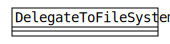
\includegraphics[width=10cm]{cdig/DelegateToFileSystem.png}
     
 一个\emph{AbstractFileSystem}的实现,其内部包装了一个FileSystem对象,
 这样使其可以利用现有的FileSystem实现。

\end{XeClass}

\begin{XeClass}{UmaskParser}
\InsertFigure{gen/UmaskParser.pdf}{UmaskParser核心成员类图}
   
 解析String中提供的八进制或符号形式的umask模式, 并返回short型整数(以八进制形式).
 Umask形式与标准形式略有不同, 它们不能指定"sticky bit"(粘滞位, 用于限制用户在公共目录中修改他人文件),
 也不能指定"special execute"(X, 拥有该标记的目录下的所有文件被无条件赋予可执行权限).

  \begin{XeMethod}{\XePublic\\ }{short}{getUMask}
       
 仅用于创建文件/目录. 符号形式的umask被用于描述"相对权限模式", 使用'+'或'-'来对
 原有的权限模式进行复位或置位.
 对八进制形式的umask而言, 指定的模式位通过创建时的模式给出.
 For octal umask, the specified bits are set in the file mode creation mask.

  \end{XeMethod}

\end{XeClass}

\begin{XeClass}{S3Exception}
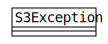
\includegraphics[width=\textwidth]{cdig/S3Exception.png}
     
 Thrown if there is a problem communicating with Amazon S3.

\end{XeClass}

\begin{XeClass}{RawLocalFs}
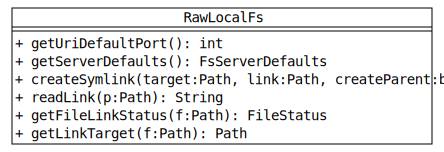
\includegraphics[width=\textwidth]{cdig/RawLocalFs.png}
    
    \begin{XeMethod}{\XeProtected}{int}{getUriDefaultPort}
         
 返回URI默认端口

    \end{XeMethod}

    \begin{XeMethod}{\XeProtected}{FsServerDefaults}{getServerDefaults}
         
 返回默认服务器

    \end{XeMethod}

    \begin{XeMethod}{\XeProtected}{void}{createSymlink}
         
 建立符号连接
 符号链接一般用于将一个文件或这个目录结构移动到系统中的另一个位置

    \end{XeMethod}

    \begin{XeMethod}{\XePrivate}{String}{readLink}
         
 读取建立的符号连接

    \end{XeMethod}

    \begin{XeMethod}{\XeProtected}{FileStatus}{getFileLinkStatus}
         
 获取文件连接状态

    \end{XeMethod}

    \begin{XeMethod}{\XeProtected}{Path}{getLinkTarget}
         
 获取连接目标

    \end{XeMethod}

\end{XeClass}

\begin{XeClass}{ChmodParser}
\includegraphics[width=\textwidth]{cdig/ChmodParser.png}
     
 解析来自chmod命令的权限格式, 并将之应用到文件系统.

    \begin{XeMethod}{\XePublic}{short}{applyNewPermission}
         
 为特定文件应用权限, 并判断应用后该文件的新的权限模式.

    \end{XeMethod}

\end{XeClass}

\begin{XeClass}{FsUrlStreamHandlerFactory}
\includegraphics[width=10cm]{cdig/FsUrlStreamHandlerFactory.png}
     
 FsUrlStreamHandlerFactory是由多个URL流输入输出处理器组成的工厂方法,
 实现了URLStreamHandlerFactory接口,
 拥有三个私有的成员变量: Configuration对象conf,
 HashMap<String, Boolean>对象 protocols,
 还有private java.net.URLStreamHandler对象handler.
 在众多的类中只有一个处理器的工作是生成UrlConnections对象,
 UrlConnections类依赖于FileSystem并选择合适的接口进行实现.
 在createURLStreamHandler方法中返回handler之前,
 需要FileSystem类的实现接口中明确清楚传入需要的参数

    \begin{XeMethod}{\XePublic}{FsUrlStreamHandlerFactory}{FsUrlStreamHandlerFactory}
         
 FsUrlStreamHandlerFactory第一个构造函数
 conf引用到一个新创建的Configuration类对象中
 确定了conf的值后调用FsUrlStreamHandler
 并将返回值赋值给handler

    \end{XeMethod}

    \begin{XeMethod}{\XePublic}{FsUrlStreamHandlerFactory}{FsUrlStreamHandlerFactory}
         
 FsUrlStreamHandlerFactory第二个构造函数
 conf引用到一个配置好的Configuration类对象中
 确定了conf的值后调用FsUrlStreamHandler
 并将返回值赋值给handler

    \end{XeMethod}

    \begin{XeMethod}{\XePublic}{java.net.URLStreamHandler}{createURLStreamHandler}
         
 FsUrlStreamHandlerFactory第二个构造函数
 createURLStreamHandler接收一个String参数protocol
 判断protocols字典中是否存在这个protocol
 若存在则将handler变量返回,不然则返回null

    \end{XeMethod}

\end{XeClass}

\begin{XeClass}{FTPException}
\InsertFigure{gen/FTPException.pdf}{FTPException核心成员类图}
   
 这个类封装了\emph{Throwable} Throwable对象用于抛出指定异常
 FTPException继承自RuntimeException,final修饰了静态变量serialVersionUID = 1L

  \begin{XeMethod}{\XePublic\\ }{FTPException}{FTPException}
       
 通过传入message,调用父类方法抛出异常

  \end{XeMethod}

  \begin{XeMethod}{\XePublic\\ }{FTPException}{FTPException}
       
 通过传入t,调用父类方法抛出异常

  \end{XeMethod}

  \begin{XeMethod}{\XePublic\\ }{FTPException}{FTPException}
       
 通过传入t,调用父类方法抛出异常

  \end{XeMethod}

\end{XeClass}

\begin{XeClass}{BufferedFSInputStream}
\includegraphics[width=\textwidth]{cdig/BufferedFSInputStream.png}
     
 BufferedFSInputStream继承了\emph{BufferedInputStream},
 通过缓存来优化其内包装的对象\emph{FSInputStream}的读取

    \begin{XeMethod}{\XePublic}{BufferedFSInputStream}{BufferedFSInputStream}
         
 创建一个指定buffer大小为size的\emph{BufferedFSInputStream}

    \end{XeMethod}

    \begin{XeMethod}{\XePublic}{void}{seek}
         
 如果要移动到的目标读取位置在目前的buffer中,那么优化他,直接在
 buffer内移动读取位置。

    \end{XeMethod}

    \begin{XeMethod}{\XePublic}{boolean}{seekToNewSource}
         
 将输入源切换到一个新的输入源,并且将偏移量移动到\emph{pos}。
 此方法在FTP、S3、Local等文件系统上均无实现(直接返回false),现有
 的唯一实现在\emph{org.apache.hadoop.hdfs.DFSInputStream.seekToNewSource(long targetPos)},其功能是在当前读取的Block失效时,切换到新的Block,并且移动偏移量,操作成
 功时返回true

    \end{XeMethod}

\end{XeClass}

\begin{XeClass}{FileAlreadyExistsException}
\InsertFigure{gen/FileAlreadyExistsException.pdf}{FileAlreadyExistsException核心成员类图}
   
 此异常使用环境为,任意操作的目标文件已存在,而且相关配置中
 并未标记文件可覆盖。

\end{XeClass}

\begin{XeClass}{FsServerDefaults}
\includegraphics[width=10cm]{cdig/FsServerDefaults.png}
     
 文件系统默认服务器类,
 向客户端提供服务器的默认相关设置参数,包括数据块的大小,
 校验和的位数,Packet的大小,文件的副本的数量,
 文件缓冲区的大小

    \begin{XeMethod}{\XePublic}{void}{write}
         
 将服务器的参数值写到输出缓存中

    \end{XeMethod}

    \begin{XeMethod}{\XePublic}{void}{readFields}
         
 读入服务器的各参数值

    \end{XeMethod}

\end{XeClass}

\begin{XeClass}{LocalFileSystem}
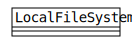
\includegraphics[width=10cm]{cdig/LocalFileSystem.png}
     
 本地文件系统,是对校验和文件系统的具体实现
 主要方法包括寻找文件、复制文件、报告检验和错误等。

\end{XeClass}

\begin{XeClass}{NativeFileSystemStore}
\includegraphics[width=10cm]{cdig/NativeFileSystemStore.png}
     
 <p>
 An abstraction for a key-based \emph{File} store.
 </p>

\end{XeClass}

\begin{XeClass}{Seekable}
\InsertFigure{gen/Seekable.pdf}{Seekable核心成员类图}
   
 此接口表示实现该接口的类具有seek方法,具备随机文件读写的能力

  \begin{XeMethod}{}{void}{seek}
       
 从文件的开始位置按给出的偏移量开始查找
 下一次read()会从偏移位置开始查找
 不能查找超过文件尾

  \end{XeMethod}

  \begin{XeMethod}{}{long}{getPos}
       
 返回当前距离文件开始位置的偏移量

  \end{XeMethod}

  \begin{XeMethod}{}{boolean}{seekToNewSource}
       
 查找数据的不同备份
 查找到新的文件返回true,否者返回false

  \end{XeMethod}

\end{XeClass}

\begin{XeClass}{KFSConfigKeys}
\includegraphics[width=10cm]{cdig/KFSConfigKeys.png}
     
 This class contains constants for configuration keys used
 in the kfs file system. 

\end{XeClass}

\begin{XeClass}{ChecksumException}
\includegraphics[width=10cm]{cdig/ChecksumException.png}
     
 抛出Checksum的错误,ChecksumException继承自IOException,
 记录一个字符串和常数,将字符串作为参数传入父类的构造器,

\end{XeClass}

\begin{XeClass}{PositionedReadable}
\includegraphics[width=10cm]{cdig/PositionedReadable.png}
     
 实现该接口的流允许从某个位置开始读的

    \begin{XeMethod}{\XePublic}{int}{read}
         
 从文件给定的位置读入指定数量的byte数, 并返回读入的byte数
 这不会改变当前文件的偏移量,并且是线程安全的.

    \end{XeMethod}

    \begin{XeMethod}{\XePublic}{void}{readFully}
         
 从文件给定的位置读入指定数量的byte数
 这不会改变当前文件的偏移量,并且是线程安全的.

    \end{XeMethod}

    \begin{XeMethod}{\XePublic}{void}{readFully}
         
 从给定的位置读入与缓存区长度相同的byte数.
 这不会改变当前文件的偏移量,并且是线程安全的.

    \end{XeMethod}

\end{XeClass}

\begin{XeClass}{ChecksumFs}
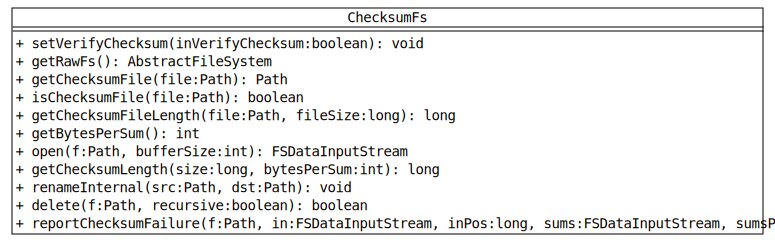
\includegraphics[width=10cm]{cdig/ChecksumFs.png}
     
 HDFS 会对写入的所有数据计算校验和(checksum),并在读取数据时验证校验和。
 针对指定字节的数目计算校验和。字节数默认是512 字节,可以通过io.bytes.per.checksum属性设置。
 通过CRC-32编码后为4字节。
 Datanode 在保存数据前负责验证checksum。
 client 会把数据和校验和一起发送到一个由多个datanode 组成的队列中,
 最后一个Datanode 负责验证checksum。
 如果验证失败,会抛出一个ChecksumException。客户端需要处理这种异常。
 客户端从datanode读取数据时,也会验证checksum。
 每个Datanode 都保存了一个验证checksum的日志。
 每次客户端成功验证一个数据块后,都会告知datanode,datanode会更新日志。
 每个datanode 也会在一个后台线程中运行一个DataBlockScanner,
 定期验证这个 datanode 上的所有数据块。
 在用Hadoop fs get命令读取文件时,可以用-ignoreCrc忽略验证。
 如果是通过FileSystem API 读取时,可以通过setVerifyChecksum(false),忽略验证。
 
 抽象检验文件系统 从文件系统过滤器类继承
 提供一个基本的文件校验系统的实现
 在客户端生成并且检验检验和,检验数据的完整性
 每个512byte的数据,生成一个4byte的检验和
 冗余备份的情况下,多个节点储存,以防止校验和本身损坏

    \begin{XeMethod}{\XePublic}{void}{setVerifyChecksum}
         
 布尔值 设置是否检验了校验和

    \end{XeMethod}

    \begin{XeMethod}{\XePublic}{AbstractFileSystem}{getRawFs}
         
 获取初始的文件系统

    \end{XeMethod}

    \begin{XeMethod}{\XePublic}{Path}{getChecksumFile}
         
 返回检验和文件关联文件的文件名

    \end{XeMethod}

    \begin{XeMethod}{\XePublic}{boolean}{isChecksumFile}
         
 当文件名是校验和文件名时,返回真值

    \end{XeMethod}

    \begin{XeMethod}{\XePublic}{long}{getChecksumFileLength}
         
 返回校验和文件的长度和源文件的大小

    \end{XeMethod}

    \begin{XeMethod}{\XePublic}{int}{getBytesPerSum}
         
 返回每个校验和的byte数

    \end{XeMethod}

    \begin{XeMethod}{\XePublic}{FSDataInputStream}{open}
         
 在指定的路径下开启一个FSData的输入流

    \end{XeMethod}

    \begin{XeMethod}{\XePublic}{long}{getChecksumLength}
         
 按byte计算校验和文件的长度

    \end{XeMethod}

    \begin{XeMethod}{\XePublic}{void}{renameInternal}
         
 重命名 files/dirs

    \end{XeMethod}

    \begin{XeMethod}{\XePublic}{boolean}{delete}
         
 在校验和文件系统中执行delete(Path, boolean)

    \end{XeMethod}

    \begin{XeMethod}{\XePublic}{boolean}{reportChecksumFailure}
         
 给文件系统报告一个校验和的错误

    \end{XeMethod}

    \begin{XeInnerClass}{ChecksumFSInputChecker}
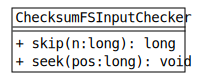
\includegraphics[width=10cm]{cdig/ChecksumFSInputChecker.png}
         
 open()方法的FS输入流
 确认数据和检验和是否匹配

        \begin{XeMethod}{\XePublic \\ \XeSync}{long}{skip}
             
 忽略或者弃用输入流中n byte的数据
 在总计忽略或者弃用n byte的数据前,用Skip方法忽略一些小的bytes
 实际忽略的byte数会被返回。如果n是负数,则不忽略任何byte。

        \end{XeMethod}

        \begin{XeMethod}{\XePublic \\ \XeSync}{void}{seek}
             
 在流中查找给定的位置
 下一次read()从此位置开始
 <p>此方法不允许搜索超过文件末,会抛出IOException

        \end{XeMethod}

    \end{XeInnerClass}
    \begin{XeInnerClass}{ChecksumFSOutputSummer}
\includegraphics[width=10cm]{cdig/ChecksumFSOutputSummer.png}
         
 给校验过的文件提供一个输出流
 为数据生成检验和.

    \end{XeInnerClass}
\end{XeClass}

\begin{XeClass}{FsConfig}
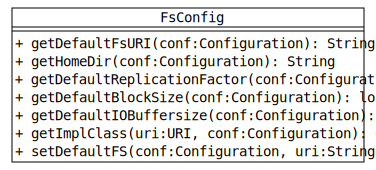
\includegraphics[width=10cm]{cdig/FsConfig.png}
     
 这个类保存了文件相关的一些Key,并且对外提供简单的借口,
 来实现设置或者获取Configuration对象的内容

    \begin{XeMethod}{\XePublic}{String}{getDefaultFsURI}
         
 获取默认的文件系统路径

    \end{XeMethod}

    \begin{XeMethod}{\XePublic}{String}{getHomeDir}
         
 获取文件系统的home文件目录

    \end{XeMethod}

    \begin{XeMethod}{\XePublic}{short}{getDefaultReplicationFactor}
         
 获取默认的文件副本数量

    \end{XeMethod}

    \begin{XeMethod}{\XePublic}{long}{getDefaultBlockSize}
         
 获取默认的文件块的大小

    \end{XeMethod}

    \begin{XeMethod}{\XePublic}{int}{getDefaultIOBuffersize}
         
 获取默认的Buffer的大小

    \end{XeMethod}

    \begin{XeMethod}{\XePublic}{Class<?>}{getImplClass}
         
 获取文件Scheme对应的类

    \end{XeMethod}

    \begin{XeMethod}{\XePublic}{void}{setDefaultFS}
         
 Setters: 功能都对应上面的Getters

    \end{XeMethod}

\end{XeClass}

\input{gen/IFSImpl}
\begin{XeClass}{S3NativeFileSystemConfigKeys}
\includegraphics[width=10cm]{cdig/S3NativeFileSystemConfigKeys.png}
     
 This class contains constants for configuration keys used
 in the s3 file system. 

\end{XeClass}

\begin{XeClass}{FtpFs}
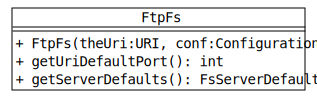
\includegraphics[width=10cm]{cdig/FtpFs.png}
     
 FTPFs是AbstractFileSystem以抽象的形式向Hadoop FS中具体的文件系统提供的实现接口
 DelegateToFileSystem是代理类
 FTPFs通过继承DelegateToFileSystem类,为旧式的文件系统提供了代理接口

    \begin{XeMethod}{}{FtpFs}{FtpFs}
         
 构造函数需要链接到上层抽象类AbstractFileSystem的URL和Configuration\emph{AbstractFileSystem.createFileSystem(URI,Configuration)}.

    \end{XeMethod}

    \begin{XeMethod}{\XeProtected}{int}{getUriDefaultPort}
         
 返回FTP的默认端口

    \end{XeMethod}

    \begin{XeMethod}{\XeProtected}{FsServerDefaults}{getServerDefaults}
         
 返回FtpConfigKeys类的getServerDefaults()方法的返回值,返回值是一个FsServerDefaults对象.

    \end{XeMethod}

\end{XeClass}

\begin{XeClass}{NativeS3FileSystem}
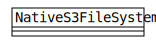
\includegraphics[width=10cm]{cdig/NativeS3FileSystem.png}
     
 <p>
 A \emph{FileSystem} for reading and writing files stored on
 <a href="http://aws.amazon.com/s3">Amazon S3</a>.
 Unlike \emph{org.apache.hadoop.fs.s3.S3FileSystem} this implementation
 stores files on S3 in their
 native form so they can be read by other S3 tools.
 A note about directories. S3 of course has no "native" support for them.
 The idiom we choose then is: for any directory created by this class,
 we use an empty object "#{dirpath}_$folder$" as a marker.
 Further, to interoperate with other S3 tools, we also accept the following:
 - an object "#{dirpath}/' denoting a directory marker
 - if there exists any objects with the prefix "#{dirpath}/", then the
 directory is said to exist
 - if both a file with the name of a directory and a marker for that
 directory exists, then the *file masks the directory*, and the directory
 is never returned.
 </p>



\end{XeClass}

\begin{XeClass}{S3FileSystemConfigKeys}
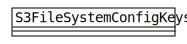
\includegraphics[width=\textwidth]{cdig/S3FileSystemConfigKeys.png}
     
 This class contains constants for configuration keys used
 in the s3 file system. 

\end{XeClass}

\begin{XeClass}{FileContext}
\includegraphics[width=10cm]{cdig/FileContext.png}
     
 FileContext为应用程序开发者提供访问Hadoop FS的接口。FileContext提供了诸如创建、
 打开、枚举目录元素(同ls)等方法。
 
 Hadoop FS支持URI命名空间(a name space)和URI文件名(names)。
 它为文件系统提供一个可以用完全限定的URI引用的森林。
 两个人通用的Hadoop FS的实现是:
 \begin{XeDuoLineTabular}{类型}{URI范例}
 \XeDLTItem{本地文件系统}{file:///path}
 \XeDLTItem{HDFS}{hdfs://nnAddress:nnPort/path}
 \end{XeDuoLineTabular}
 
 URI十分灵活,但却要求用户知晓服务器的名字或者地址才可以。
 简便起见,开发者通常会希望在特定环境下访问默认文件系统而忽略服务器的名字或者地址。
 此举还有一个额外的好处,即是,它允许用户修改自己的默认文件系统(比如,管理员将应用从
 集群1迁移至集群2)。
 
 为了实现这一目的,Hadoop支持默认文件系统记号(notion)。
 即使默认文件系统的设置通常由默配置给出,用户仍然可以设置自己的文件系统。
 一个默认文件系统意味着体系(scheme)和权限,'/'分隔的相对路径
 会被解析成相对于默认文件系统的路径。

    \begin{XeInnerClass}{Util}
\includegraphics[width=10cm]{cdig/Util.png}
         
 Utility/library methods built over the basic FileContext methods.
 Since this are library functions, the oprtation are not atomic
 and some of them may partially complete if other threads are making
 changes to the same part of the name space.

    \end{XeInnerClass}

    \begin{XeInnerClass}{FileContextFinalizer}
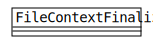
\includegraphics[width=10cm]{cdig/FileContextFinalizer.png}
         
 Deletes all the paths in deleteOnExit on JVM shutdown.

    \end{XeInnerClass}
    \begin{XeInnerClass}{FSLinkResolver}
\includegraphics[width=10cm]{cdig/FSLinkResolver.png}
         
 Class used to perform an operation on and resolve symlinks in a
 path. The operation may potentially span multiple file systems.

    \end{XeInnerClass}
\end{XeClass}

\input{gen/KFSInputStream}
\begin{XeClass}{UnsupportedFileSystemException}
\includegraphics[width=\textwidth]{cdig/UnsupportedFileSystemException.png}
     
 此异常的出现情况是,请求的文件系统或者文件scheme不被支持

\end{XeClass}

\begin{XeClass}{FileSystemStore}
\includegraphics[width=10cm]{cdig/FileSystemStore.png}
     
 A facility for storing and retrieving \emph{INode}s and \emph{Block.}s.

\end{XeClass}

\begin{XeClass}{FSDataInputStream}
\includegraphics[width=\textwidth]{cdig/FSDataInputStream.png}
     
 一个包装类,类似于\emph{DataInputStream}, 里面包装了一个
 实现了\emph{Seekable}和\emph{PositionReadbale}接口的{@link java.io.InputStream},通常是传入 {@link FSInputStream.},
 此类的方法都是通过调用被包装对象的对应方法来实现的。

\end{XeClass}

\begin{XeClass}{BlockLocation}
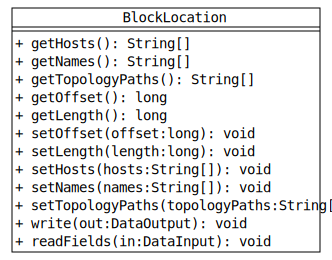
\includegraphics[width=\textwidth]{cdig/BlockLocation.png}
     
 \emph{BlockLocation}是块位置类.
 域包含主机号、端口号、拓扑路径以及偏移量和长度信息
 主要方法为域的get、set方法和实现Writable接口的读写方法

    \begin{XeMethod}{\XePublic}{String[]}{getHosts}
         
 获取主机名列表

    \end{XeMethod}

    \begin{XeMethod}{\XePublic}{String[]}{getNames}
         
 获取端口号列表

    \end{XeMethod}

    \begin{XeMethod}{\XePublic}{String[]}{getTopologyPaths}
         
 获取每一个主机的网络拓扑路径的列表,路径的最后部分是主机

    \end{XeMethod}

    \begin{XeMethod}{\XePublic}{long}{getOffset}
         
 获取块的偏移量

    \end{XeMethod}

    \begin{XeMethod}{\XePublic}{long}{getLength}
         
 获取块的长度信息

    \end{XeMethod}

    \begin{XeMethod}{\XePublic}{void}{setOffset}
         
 设置快的偏移量

    \end{XeMethod}

    \begin{XeMethod}{\XePublic}{void}{setLength}
         
 设置块的长度信息

    \end{XeMethod}

    \begin{XeMethod}{\XePublic}{void}{setHosts}
         
 设置当前块的主机名

    \end{XeMethod}

    \begin{XeMethod}{\XePublic}{void}{setNames}
         
 设置当前块的端口号

    \end{XeMethod}

    \begin{XeMethod}{\XePublic}{void}{setTopologyPaths}
         
 设置主机的网络拓扑路径

    \end{XeMethod}

    \begin{XeMethod}{\XePublic}{void}{write}
         
 实现Writable的write方法,主要是将块位置的
 各参数信息写到输出缓存中

    \end{XeMethod}

    \begin{XeMethod}{\XePublic}{void}{readFields}
         
 实现Writable的readFields方法
 读入块位置的各参数信息

    \end{XeMethod}

\end{XeClass}

\input{gen/KFSImpl}
\begin{XeClass}{FTPFileSystem}
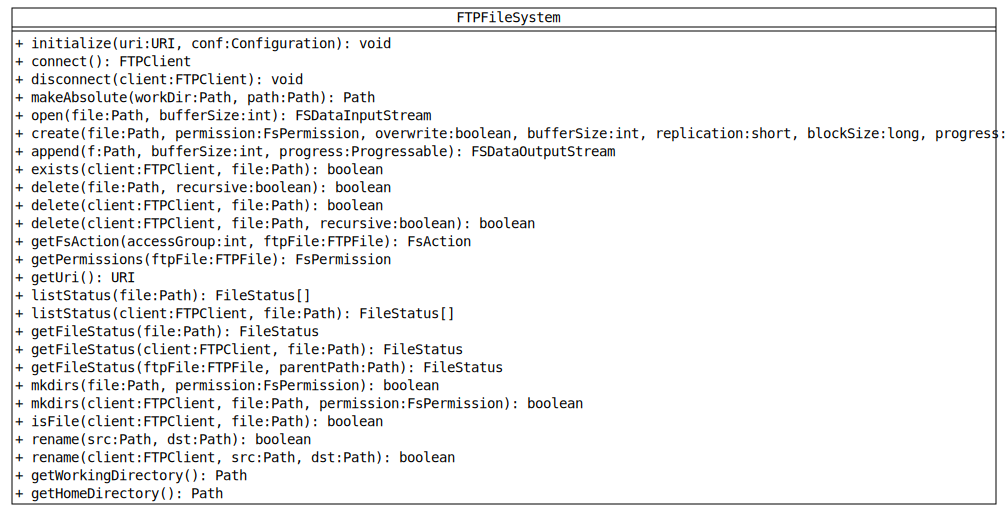
\includegraphics[width=10cm]{cdig/FTPFileSystem.png}
     
 由FTP服务器支持的文件系统,基于FTP协议和FTP服务器交互的FileSystem API实现
 继承自\emph{FileSystem}

    \begin{XeMethod}{\XePublic}{void}{initialize}
         
 使用超类FileSystem调用initialize,通过uri获得host,port,和userAndPassword
 初始化的函数通过获得的host,port,user,password配置Configuration对象.
 host通过Configuration对象设置保存在fs.ftp.host
 port通过Configuration对象设置保存在fs.ftp.host.port
 user通过Configuration对象设置保存在"fs.ftp.user." + host
 password通过Configuration对象设置保存在"fs.ftp.password." + host

    \end{XeMethod}

    \begin{XeMethod}{\XePrivate}{FTPClient}{connect}
         
 使用获取得到的Configuration配置FTP Server
 通过在从初始化里保存好的host,port,user,password获取相应的值
 使用FTPClient类生成FTPClient对象,并通过给定主机地址和端口号进行连接
 使用FTPClient对象和从Configuration对象中取出的user和password Sign In
 设置FTP.BLOCK_TRANSFER_MODE,FTP.BINARY_FILE_TYPE and DEFAULT_BUFFER_SIZE

    \end{XeMethod}

    \begin{XeMethod}{\XePrivate}{void}{disconnect}
         
 FTPFileSystem类断开连接API
 判断FTPClient对象是否为null,不为null则进一步判断是否没有连接
 当判断为有连接,则通过FTPClient调用disconnect方法断开连接
 logoutSuccess记录断开连接登出的状态,判断是否断开连接成功

    \end{XeMethod}

    \begin{XeMethod}{\XePrivate}{Path}{makeAbsolute}
         
 通过给定workDir工作目录和path路径

    \end{XeMethod}

    \begin{XeMethod}{\XePublic}{FSDataInputStream}{open}
         
 open函数接收两个参数,Path对象file和基本数据类型int bufferSize
 获得连接的FTPClient对象,并得到工作目录的绝对路径
 判断fileStat是不是一个目录,若是则断开FTPClient对象client连接
 通过client获得bufferSize大小的字节数
 获得当前工作目录的父路径,只有这样才能在使用InputStream状态下读
 当在FSDataInputStream内调用close()方法,FTPClient对象断开连接
 当FTPClient对象处于inconsistent状态,则要在FTP Server端登出和断开连接,并关闭文件流操作

    \end{XeMethod}

    \begin{XeMethod}{\XePublic}{FSDataOutputStream}{create}
         
 create方法获得连接的FTPClient对象,并得到工作目录的绝对路径
 判断client对象是否存在file路径并判断是否被重写了,若存在,并重写了则删了这个路径,不然则断开FTPClient连接
 抛出异常IOException("File already exists: " + file)
 获得当前工作目录的父路径,若没有父路径或者无法在父路径中有可写准许,则断开FTPClient连接
 通过client获得bufferSize大小的字节数
 当在FSDataInputStream内FTPClient对象调用close()方法,FTPClient对象断开连接
 当FTPClient对象处于inconsistent状态,则要在FTP Server端登出和断开连接,并关闭文件流操作

    \end{XeMethod}

    \begin{XeMethod}{\XePublic}{FSDataOutputStream}{append}
         
 append方法目前尚不支持 

    \end{XeMethod}

    \begin{XeMethod}{\XePrivate}{boolean}{exists}
         
 exists方法可以不需要打开一个新的连接可以判断FTPClient对象client是否有文件目录file

    \end{XeMethod}

    \begin{XeMethod}{\XePublic}{boolean}{delete}
         
 Override的delete方法通过传入文件目录file,当recursive为true,使用建立连接的FTPClient对象删除这个文件目录

    \end{XeMethod}

    \begin{XeMethod}{\XePrivate}{boolean}{delete}
         
 delete装饰器调用delete(Path file, boolean recursive)方法

    \end{XeMethod}

    \begin{XeMethod}{\XePrivate}{boolean}{delete}
         
 获得client的工作目录并与file组合得到文件目录的绝对路径
 获得绝对路径下的所有文件,并调用delete方法全部删除

    \end{XeMethod}

    \begin{XeMethod}{\XePrivate}{FsAction}{getFsAction}
         
 判断ftpFile与accessGroup是否有可读允许,有则将FsAction对象action赋值为FsAction.READ
 判断ftpFile与accessGroup是否有可写允许,有则将FsAction对象action赋值为FsAction.WRITE
 判断ftpFile与accessGroup是否有可操作允许,有则将FsAction对象action赋值为FsAction.EXECUTE

    \end{XeMethod}

    \begin{XeMethod}{\XePrivate}{FsPermission}{getPermissions}
         
 通过给user,group,others设置FsAction属性,创建FsPermission对象并返回

    \end{XeMethod}

    \begin{XeMethod}{\XePublic}{URI}{getUri}
         
 返回uri格式

    \end{XeMethod}

    \begin{XeMethod}{\XePublic}{FileStatus[]}{listStatus}
         
 使用FTPClient对象client获得连接,并返回当前文件目录下的文件列表

    \end{XeMethod}

    \begin{XeMethod}{\XePrivate}{FileStatus[]}{listStatus}
         
 listStatus方法也是与上述方法实现类似功能,获得当前FTPClient对象client的工作目录
 然后获取其绝对路径,最后返回绝对路径下的所有文件列表.

    \end{XeMethod}

    \begin{XeMethod}{\XePublic}{FileStatus}{getFileStatus}
         
 通过getFileStatus的参数file,获得FTPClient对象client文件目录的状态

    \end{XeMethod}

    \begin{XeMethod}{\XePrivate}{FileStatus}{getFileStatus}
         
 获取当前工作路径的绝对路径,再获得绝对路径的父路径
 若父路径不存在,则对它进行设置
 若父路径存在,则遍历其文件列表,判断是否存在ftpFile.getName()  file.getName()
 若存在则继续递归下去寻找getFileStatus(ftpFile, parentPath)

    \end{XeMethod}

    \begin{XeMethod}{\XePrivate}{FileStatus}{getFileStatus}
         
 覆盖在FTPFile\emph{FileStatus}文件目录信息
 使用默认的blockSize当FTP Client不清楚Server的Block Size

    \end{XeMethod}

    \begin{XeMethod}{\XePublic}{boolean}{mkdirs}
         
 使用FTPClient对象client获得连接,并判断是否能创建文件目录

    \end{XeMethod}

    \begin{XeMethod}{\XePrivate}{boolean}{mkdirs}
         
 通过给定的client,file和permission判断是否可以在当前工作目录的绝对路径下创建一个文件目录

    \end{XeMethod}

    \begin{XeMethod}{\XePrivate}{boolean}{isFile}
         
 通过调用getFileStatus(client, file).isFile()方法判断当前client实例在file目录下是否存在文件目录

    \end{XeMethod}

    \begin{XeMethod}{\XePublic}{boolean}{rename}
         
 调用 rename(FTPClient client, Path src, Path dst)函数,并返回结果

    \end{XeMethod}

    \begin{XeMethod}{\XePrivate}{boolean}{rename}
         
 获取src的绝对路径和dst的绝对路径,若src的绝对路径的父路径与dst的不相等,则无法重命名
 重命名成功后则返回true

    \end{XeMethod}

    \begin{XeMethod}{\XePublic}{Path}{getWorkingDirectory}
         
 调用getHomeDirectory()返回home文件路径

    \end{XeMethod}

    \begin{XeMethod}{\XePublic}{Path}{getHomeDirectory}
         
 返回当前工作目录Path

    \end{XeMethod}

\end{XeClass}

\begin{XeClass}{CommonConfigurationKeys}
\includegraphics[width=10cm]{cdig/CommonConfigurationKeys.png}
     
 此类包含HadoopCommon中配置文件的所有键的键值,以静态public成员的方式提供。

\end{XeClass}

\begin{XeClass}{FsUrlConnection}
\includegraphics[width=\textwidth]{cdig/FsUrlConnection.png}
     
 URL连接到InputStreams上的类
 具有Configuration对象conf和InputStream对象is作为实例属性
 继承自URLConnection的connect方法和getInputStream方法,并Override覆盖其原来方法
 构造函数接收两个参数,第一个参数是Configuration conf.
 第二个参数是URL对象url,调用其超类URLConnection构造函数super(url)

    \begin{XeMethod}{\XePublic}{void}{connect}
         
 connect方法是继承自URLConnection,在FsUrlConnection类中Override的方法
 该方法通过FileSystem.get(url.toURI(), conf)方法获得FileSystem对象fs
 并用fs打开url的地址获得的输入流对象赋值给FsUrlConnection类的实例变量is

    \end{XeMethod}

    \begin{XeMethod}{\XePublic}{InputStream}{getInputStream}
         
 getInputStream()方法是继承自URLConnection,在FsUrlConnection类中Override的方法
 该方法首先判断FsUrlConnection类的实例变量is是否为null,若为null则调用connect方法

    \end{XeMethod}

\end{XeClass}

\begin{XeClass}{S3Credentials}
\includegraphics[width=\textwidth]{cdig/S3Credentials.png}
     
 <p>
 Extracts AWS credentials from the filesystem URI or configuration.
 </p>

\end{XeClass}

\begin{XeClass}{FsShell}
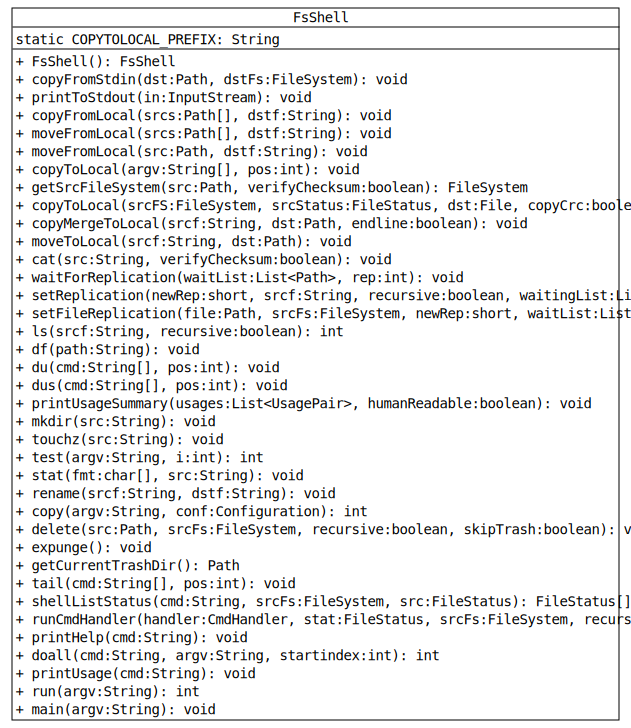
\includegraphics[width=\textwidth]{cdig/FsShell.png}
     
 向HFS中的文件系统提供命令行访问接口. 

    \begin{XeMethod}{\XePublic}{FsShell}{FsShell}
         
 以空的配置构造实例 

    \end{XeMethod}

    \begin{XeMethod}{\XePrivate}{void}{copyFromStdin}
         
 从stdin复制到指定\emph{FileSystem}的指定文件.

    \end{XeMethod}

    \begin{XeMethod}{\XePrivate}{void}{printToStdout}
         
 打印到stdout.

    \end{XeMethod}

    \begin{XeMethod}{}{void}{copyFromLocal}
         
 将本地文件添加到HFS.

    \end{XeMethod}

    \begin{XeMethod}{}{void}{moveFromLocal}
         
 从本地移动多个文件到目标文件系统.

    \end{XeMethod}

    \begin{XeMethod}{}{void}{moveFromLocal}
         
 从本地移动一个文件到目标文件系统.

    \end{XeMethod}

    \begin{XeMethod}{}{void}{copyToLocal}
         
 获取匹配模式的所有文件, 并将之复制到本地.
 源文件会被保存,当拷贝多个文件时,目标位置必须是一个文件夹,
 否则会抛出IOException异常。

    \end{XeMethod}

    \begin{XeMethod}{\XePrivate}{FileSystem}{getSrcFileSystem}
         
 返回src和conf对应的\emph{FileSystem},如果目标\emph{FileSystem.}支持校验和,则设置校验和。

    \end{XeMethod}

    \begin{XeMethod}{\XePrivate}{void}{copyToLocal}
         
 将\emph{FileSystem}中的文件拷贝到本地。

    \end{XeMethod}

    \begin{XeMethod}{}{void}{copyMergeToLocal}
         
 将符合srcf的模式的文件均拷贝到本地,合并为一个文件,源文件将被保留,
 此方法在合并时,可以指定是否在每个被合并的文件末尾加入一行来
 区分每个文件。

    \end{XeMethod}

    \begin{XeMethod}{}{void}{moveToLocal}
         
 获取并拷贝srcf指定的文件到本地目录,并且删除源文件。
 但此方法尚未被实现。

    \end{XeMethod}

    \begin{XeMethod}{}{void}{cat}
         
 获取所有的符合srcf模式的文件,并显示到\emph{stdout}

    \end{XeMethod}

    \begin{XeMethod}{}{void}{waitForReplication}
         
 等待所有的在waitlist中的文件,直到其副本数量达到rep

    \end{XeMethod}

    \begin{XeMethod}{}{void}{setReplication}
         
 改变一个文件的副本数。recursive选项用于递归改变目录下所有文件的副本数。

    \end{XeMethod}

    \begin{XeMethod}{\XePrivate}{void}{setFileReplication}
         
 为文件设置副本数量

    \end{XeMethod}

    \begin{XeMethod}{\XePrivate}{int}{ls}
         
 即unix系统上的ls命令,获取符合<i>srcf</i>模式的文件的状态

    \end{XeMethod}

    \begin{XeMethod}{}{void}{df}
         
 显示包含path的文件系统的分区大小

    \end{XeMethod}

    \begin{XeMethod}{}{void}{du}
         
 显示所有符合输入模式的文件的大小

    \end{XeMethod}

    \begin{XeMethod}{}{void}{dus}
         
 显示输入模式匹配的文件和文件目录的基本信息。

    \end{XeMethod}

    \begin{XeMethod}{\XePrivate}{void}{printUsageSummary}
         
 打印文件使用量的信息,此方法被\emph{du}命令使用。

    \end{XeMethod}

    \begin{XeMethod}{}{void}{mkdir}
         
 创建一个目录

    \end{XeMethod}

    \begin{XeMethod}{}{void}{touchz}
         
 在指定的src位置创建一个0长度的文件。
 此命令在未来版本将会仿照unix中的touch命令。

    \end{XeMethod}

    \begin{XeMethod}{}{int}{test}
         
 测试文件的类型

    \end{XeMethod}

    \begin{XeMethod}{}{void}{stat}
         
 将path的统计信息按照指定的格式输出
 格式字串:
 %b: 文件的block数量
 %n: 文件名
 %o: block大小
 %r: 副本数量
 %y: UTC 时间,格式为yyyy-MM-dd HH:mm:ss
 %Y: 毫秒数,从January 1, 1970 UTC开始

    \end{XeMethod}

    \begin{XeMethod}{}{void}{rename}
         
 移动/重命名文件,当一次移动多个文件时,目标位置必须是一个目录,否则会抛出
 \emph{IOException}

    \end{XeMethod}

    \begin{XeMethod}{\XePrivate}{int}{copy}
         
 复制文件,当一次复制多个文件时,目标位置必须是一个目录,否则会抛出

    \end{XeMethod}

    \begin{XeMethod}{\XePrivate}{void}{delete}
         
 删除src指定的文件,可以指定是否递归删除,可以指定是否移入垃圾箱

    \end{XeMethod}

    \begin{XeMethod}{\XePrivate}{void}{expunge}
         
 清空垃圾桶

    \end{XeMethod}

    \begin{XeMethod}{\XePublic}{Path}{getCurrentTrashDir}
         
 返回与这个FsShell对象相关的\emph{Trash}对象

    \end{XeMethod}

    \begin{XeMethod}{\XePrivate}{void}{tail}
         
 解析输入的命令,并执行tail命令

    \end{XeMethod}

    \begin{XeMethod}{\XePrivate}{FileStatus[]}{shellListStatus}
         
 返回src指定的文件夹所在的目录的所有文件的\emph{FileStatus}
 对象.

    \end{XeMethod}

    \begin{XeMethod}{\XePrivate}{int}{runCmdHandler}
         
 对一个CommandHandler执行其对应的命令,如果recursive选项为ture,则会递归执行

    \end{XeMethod}

    \begin{XeMethod}{\XePrivate}{void}{printHelp}
         
 根据不同的cmd来输出对应的帮助信息。

    \end{XeMethod}

    \begin{XeMethod}{\XePrivate}{int}{doall}
         
 对argv中从startindex开始的所有参数,执行cmd指定的命令。

    \end{XeMethod}

    \begin{XeMethod}{\XePrivate}{void}{printUsage}
         
 打印指定cmd的使用格式。

    \end{XeMethod}

    \begin{XeMethod}{\XePublic}{int}{run}
         
 Shell命令的主要处理函数,该函数会根据输入指令的不同,调用具体的处理函数。

    \end{XeMethod}

    \begin{XeMethod}{\XePublic}{void}{main}
         
 hadoop文件系统Shell接口的主要入口函数

    \end{XeMethod}


    \begin{XeInnerClass}{CmdHandler}
\includegraphics[width=\textwidth]{cdig/CmdHandler.png}
         
 该类会在给定的\emph{FileStatus}对象上运行,可以
 被用来执行chmod,chown等多种操作。
 例如在\emph{FsShellPermissions}类中,此类
 被继承为\emph{ChmodHandler</code>和<code>CmdHandler}

    \end{XeInnerClass}
    \begin{XeInnerClass}{DelayedExceptionThrowing}
\includegraphics[width=\textwidth]{cdig/DelayedExceptionThrowing.png}
         
 该类的作用是累积发生的Exception,等到指定的时间再进行抛出。
 例如在ls命令中,首先会逐条显示文件的信息,然后再抛出异常。

    \end{XeInnerClass}
    \begin{XeInnerClass}{UsagePair}
\includegraphics[width=\textwidth]{cdig/UsagePair.png}
         
 工具类,用作du的输出

    \end{XeInnerClass}
\end{XeClass}

\begin{XeClass}{CommandUtils}
\includegraphics[width=\textwidth]{cdig/CommandUtils.png}
     
 该类仅提供一个用于格式化用法说明的静态方法.

\end{XeClass}

\begin{XeClass}{UnresolvedLinkException}
\InsertFigure{gen/UnresolvedLinkException.pdf}{UnresolvedLinkException核心成员类图}
   
 UnresolvedLinkException继承自IOException异常类
 有一个静态常量serialVersionUID = 1L
 UnresolvedLinkException()方法和UnresolvedLinkException(String msg)均调用父类方法

\end{XeClass}

\begin{XeClass}{INode}
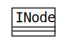
\includegraphics[width=10cm]{cdig/INode.png}
     
 Holds file metadata including type (regular file, or directory),
 and the list of blocks that are pointers to the data.

\end{XeClass}

\begin{XeClass}{FsShellPermissions}
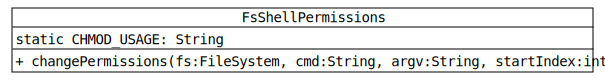
\includegraphics[width=10cm]{cdig/FsShellPermissions.png}
     
 FsShellPermissions类是将文件操作与命令行关联起来的类
 因为FsShell类越来越大,所以将FsShellPermissions类单独分离出来
 FsShellPermissions类中有三个静态内部类,分别是ChmodHandler,ChownHandler和ChgrpHandler
 还有一个静态方法changePermissions,将三个静态内部类的情况与命令行关联起来使用

    \begin{XeMethod}{}{int}{changePermissions}
         
 静态方法changePermissions,将三个静态内部类的情况与命令行关联起来使用
 当cmd匹配上-chmod,调用ChmodHandler(fs, argv[startIndex++])构造函数并将对象赋值给handler
 当cmd匹配上-chown,调用ChownHandler(fs, argv[startIndex++])构造函数并将对象赋值给handler
 当cmd匹配上-chgrp,调用ChgrpHandler(fs, argv[startIndex++])构造函数并将对象赋值给handler

    \end{XeMethod}

    \begin{XeInnerClass}{ChmodHandler}
\includegraphics[width=10cm]{cdig/ChmodHandler.png}
        
        \begin{XeMethod}{}{ChmodHandler}{ChmodHandler}
             
 ChmodHandler继承自CmdHandler,ChmodHandler构造函数调用父类的构造函数并传入"chmod"和fs
 同时传入modeStr生成ChmodParser对象赋值给FsShellPermissions类的静态变量ChmodParser pp

        \end{XeMethod}

        \begin{XeMethod}{\XePrivate}{void}{patternError}
             
 当模式发生错误匹配不上时候抛出带有特定信息异常

        \end{XeMethod}

        \begin{XeMethod}{\XePublic}{void}{run}
             
 Override父类run方法从ChmodParser对象pp获得权限(写入权限,读取权限,操作权限)

        \end{XeMethod}

    \end{XeInnerClass}
    \begin{XeInnerClass}{ChownHandler}
\includegraphics[width=10cm]{cdig/ChownHandler.png}
        
        \begin{XeMethod}{\XeProtected}{ChownHandler}{ChownHandler}
             
 ChownHandler继承自CmdHandler,protected继承ChownHandler构造函数调用父类的构造函数并传入cmd和fs

        \end{XeMethod}

        \begin{XeMethod}{}{ChownHandler}{ChownHandler}
             
 ChownHandler继承自CmdHandler,ChownHandler构造函数调用父类的构造函数并传入"chown"和fs
 chownPattern使用正则表达式匹配ownerStr并赋值给matcher,mathcer内部存有若干组匹配上的结果
 将第二组matcher.group(1)结果赋值给这个类的owner,将第四组结果matcher.group(3)赋值给这个类的group

        \end{XeMethod}

        \begin{XeMethod}{\XePublic}{void}{run}
             
 通过从file.getOwner()和file.getGroup()中取值分别与owner和group比较
 并将结果分别赋值给newOwner和newGroup
 当newOwner和newGroup其中一个为空,则从file.getOwner()和file.getGroup()取值
 在srcFs中调用setOwner(file.getPath(), newOwner, newGroup)方法

        \end{XeMethod}

    \end{XeInnerClass}
    \begin{XeInnerClass}{ChgrpHandler}
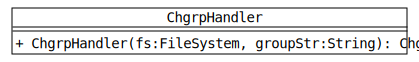
\includegraphics[width=10cm]{cdig/ChgrpHandler.png}
        
        \begin{XeMethod}{}{ChgrpHandler}{ChgrpHandler}
             
 ChgrpHandler继承自ChownHandler,ChgrpHandler构造函数调用父类的构造函数并传入chgrp和fs
 chgrpPattern使用正则表达式匹配groupStr并赋值给matcher,mathcer内部存有若干组匹配上的结果
 将第二组结果matcher.group(1)赋值给这个类的group

        \end{XeMethod}

    \end{XeInnerClass}
\end{XeClass}

\begin{XeClass}{FtpConfigKeys}
\includegraphics[width=10cm]{cdig/FtpConfigKeys.png}
     
 这个类包含了使用final修饰的配置关键变量,用于这个FTP File System

\end{XeClass}

\begin{XeClass}{DF}
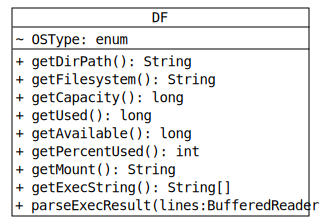
\includegraphics[width=10cm]{cdig/DF.png}
    
    \begin{XeMethod}{\XePublic}{String}{getDirPath}
         
 返回正在检查的规范路径所指的位置

    \end{XeMethod}

    \begin{XeMethod}{\XePublic}{String}{getFilesystem}
         
 返回一个字符串,指示正在检查的文件系统

    \end{XeMethod}

    \begin{XeMethod}{\XePublic}{long}{getCapacity}
         
 返回文件系统的总字节数

    \end{XeMethod}

    \begin{XeMethod}{\XePublic}{long}{getUsed}
         
 返回文件系统的已用字节数

    \end{XeMethod}

    \begin{XeMethod}{\XePublic}{long}{getAvailable}
         
 返回文件系统的可用字节数

    \end{XeMethod}

    \begin{XeMethod}{\XePublic}{int}{getPercentUsed}
         
 返回文件系统中的使用百分比

    \end{XeMethod}

    \begin{XeMethod}{\XePublic}{String}{getMount}
         
 返回文件系统的挂载点

    \end{XeMethod}

    \begin{XeMethod}{\XeProtected}{String[]}{getExecString}
         
 检测命令

    \end{XeMethod}

    \begin{XeMethod}{\XeProtected}{void}{parseExecResult}
         
 解析输出

    \end{XeMethod}

\end{XeClass}

\begin{XeClass}{AccessControlException}
\includegraphics[width=\textwidth]{cdig/AccessControlException.png}
     
 与访问控制有关的异常类,继承自IOException.

    \begin{XeMethod}{\XePublic}{AccessControlException}{AccessControlException}
         
 构造函数,出现异常返回信息"Permission denied."
 Default constructor is needed for unwrapping from\emph{org.apache.hadoop.ipc.RemoteException}.

    \end{XeMethod}

\end{XeClass}

\begin{XeClass}{Count}
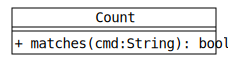
\includegraphics[width=\textwidth]{cdig/Count.png}
     
 计数目录, 文件, 字节, 限额以及限额的余量.

    \begin{XeMethod}{\XePublic}{boolean}{matches}
         
 检查一个命令是否是计数命令.

    \end{XeMethod}

\end{XeClass}

\begin{XeClass}{LocalConfigKeys}
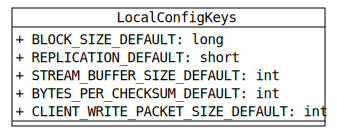
\includegraphics[width=\textwidth]{cdig/LocalConfigKeys.png}
     
 该类包含一些用在LocalFileSystem、RawLocalFs、CheckSumFs的
 配置关键字的常量

\end{XeClass}

\begin{XeClass}{Command}
\InsertFigure{gen/Command.pdf}{Command核心成员类图}
   
 用于执行文件命令的抽象类.

  \begin{XeMethod}{\XeAbstract\\ \XePublic\\ }{String}{getCommandName}
       
 删除潜在的前导字符, 返回命令名 

  \end{XeMethod}

  \begin{XeMethod}{\XeAbstract\\ \XeProtected\\ }{void}{run}
       
 在给定的路径上执行文件命令

  \end{XeMethod}

  \begin{XeMethod}{\XePublic\\ }{int}{runAll}
       
 在给定的路径簇上的执行命令, 并返回状态码

  \end{XeMethod}

\end{XeClass}

\begin{XeClass}{Syncable}
\includegraphics[width=10cm]{cdig/Syncable.png}
     
 这个接口声明了对Client的buffer进行flush的操作,此接口主要被
 BufferedIOStream实现。
 
 此接口的两个主要方法hflush、hsync的设计目的不同,hsync的目的是在执行
 完之后,保证数据
 会写在磁盘上,而hflush只会保证对数据源的新Client会读到刚flush的数据。
 
 在现在分析的HDFS版本中,这个接口的hflush和hsync方法一样,hsync会调用
 hflush。再后来2.x版本中,这两个方法将会有不同的实现。

\end{XeClass}

\input{gen/S3InputStream}
\input{gen/PathFilter}
\begin{XeClass}{FSInputChecker}
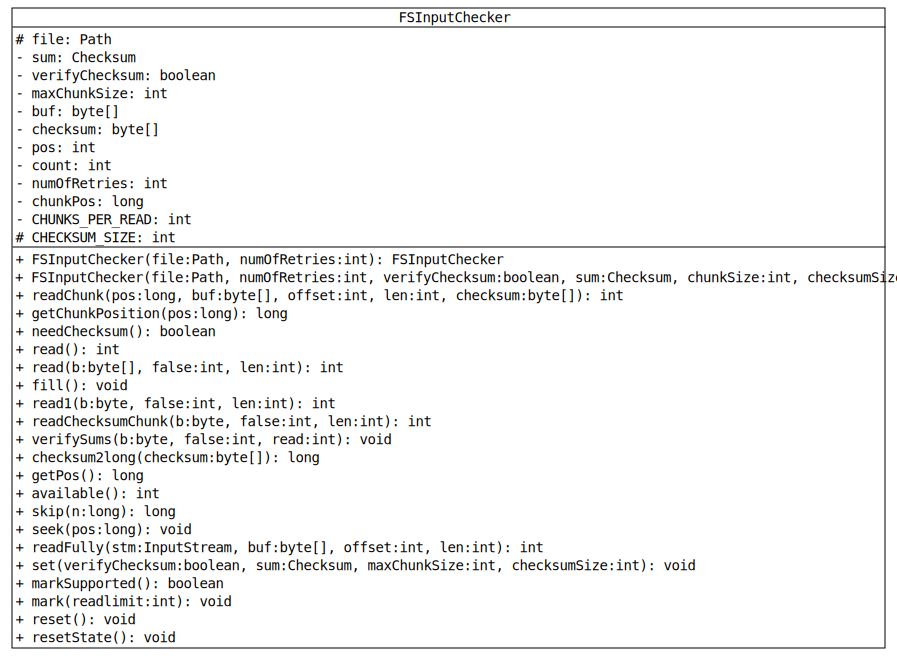
\includegraphics[width=10cm]{cdig/FSInputChecker.png}
    
    \begin{XeMethod}{\XeProtected}{FSInputChecker}{FSInputChecker}
         
 构造函数

    \end{XeMethod}

    \begin{XeMethod}{\XeProtected}{FSInputChecker}{FSInputChecker}
         
 构造函数

    \end{XeMethod}

    \begin{XeMethod}{\XeAbstract \\ \XeProtected}{int}{readChunk}
         
 从文件中读取数据和校验和,将数据放入buf,将校验和放入checksum。
 如果len不是ChunkSize的整数倍,那么将会读取少于len个字节,以保证
 读取的数据量为ChunkSize的整数倍。
 如果校验和功能被禁用,则在checksum位置传入null,并且在读取时不会
 因为len不是ChunkSize的整数倍而导致读取字节数小于len。

    \end{XeMethod}

    \begin{XeMethod}{\XeAbstract \\ \XeProtected}{long}{getChunkPosition}
         
 返回pos位置所在的Chunk

    \end{XeMethod}

    \begin{XeMethod}{\XeProtected \\ \XeSync}{boolean}{needChecksum}
         
 返回是否需要校验

    \end{XeMethod}

    \begin{XeMethod}{\XePublic \\ \XeSync}{int}{read}
         
 从当前缓冲区读取一个字节

    \end{XeMethod}

    \begin{XeMethod}{\XePublic \\ \XeSync}{int}{read}
         
 读取len个字节到字节数组b的偏移量off处,读取的数据都经过校验。
 此方法会尝试不断读取,知道读取到len个字节,直到EOF或者IOException

    \end{XeMethod}

    \begin{XeMethod}{\XePrivate}{void}{fill}
         
 向buf中填充一个经过校验的chunk

    \end{XeMethod}

    \begin{XeMethod}{\XePrivate}{int}{read1}
         
 读取len个字节到字节数组b的偏移量off处,如果len超出了Chunk的大小
 则会先向缓冲区中填入一个Chunk,再从buf复制到b中。

    \end{XeMethod}

    \begin{XeMethod}{\XePrivate}{int}{readChecksumChunk}
         
 读取一个或多个经过校验和检查的Chunk到b指定的字节数组的偏移量offset处,
 这个方法保证所有读取到的数据都是经过校验。

    \end{XeMethod}

    \begin{XeMethod}{\XePrivate}{void}{verifySums}
         
 计算字节数组b中的要进行校验的数据的校验和,并与checksum中的,即当前读取的
 chunk的校验和进行比较

    \end{XeMethod}

    \begin{XeMethod}{\XePublic}{long}{checksum2long}
         
 将一个checksum转换为一个long数字

    \end{XeMethod}

    \begin{XeMethod}{\XePublic \\ \XeSync}{long}{getPos}
         
 返回当前文件的读取位置

    \end{XeMethod}

    \begin{XeMethod}{\XePublic \\ \XeSync}{int}{available}
         
 返回当前缓冲区中尚未读取的字节。

    \end{XeMethod}

    \begin{XeMethod}{\XePublic \\ \XeSync}{long}{skip}
         
 在输入流中跳过并忽略n个字节,如果n是负数,则不会跳过任何字节。

    \end{XeMethod}

    \begin{XeMethod}{\XePublic \\ \XeSync}{void}{seek}
         
 移动读取位置到pos,下一次read将会从pos位置读取。

    \end{XeMethod}

    \begin{XeMethod}{\XeProtected}{int}{readFully}
         
 A utility function that tries to read up to \emph{len} bytes from
 \emph{stm}
 一个静态工具类,从\emph{stm</code>中读取<code>len}个字节,放入buf
 中的offset位置。

    \end{XeMethod}

    \begin{XeMethod}{\XeFinal \\ \XeProtected \\ \XeSync}{void}{set}
         
 设置校验和相关参数

    \end{XeMethod}

    \begin{XeMethod}{\XeFinal \\ \XePublic}{boolean}{markSupported}
         
 不支持mark

    \end{XeMethod}

    \begin{XeMethod}{\XeFinal \\ \XePublic}{void}{mark}
         
 不支持mark

    \end{XeMethod}

    \begin{XeMethod}{\XeFinal \\ \XePublic}{void}{reset}
         
 不支持reset

    \end{XeMethod}

    \begin{XeMethod}{\XePrivate}{void}{resetState}
         
 重置FSInputChecker的state

    \end{XeMethod}

\end{XeClass}

\begin{XeClass}{PermissionStatus}
\InsertFigure{gen/PermissionStatus.pdf}{PermissionStatus核心成员类图}
   
 存储与权限有关的状态信息.
 提供了与FsPermission对应的权限状态信息

  \begin{XeMethod}{\XePublic\\ }{PermissionStatus}{createImmutable}
       
 创建不可变的PermissionStatus实例 

  \end{XeMethod}

  \begin{XeMethod}{\XePublic\\ }{String}{getUserName}
       
 Return user name
 获取文件所属者名字

  \end{XeMethod}

  \begin{XeMethod}{\XePublic\\ }{String}{getGroupName}
       
 Return group name
 获取文件所属组的名字

  \end{XeMethod}

  \begin{XeMethod}{\XePublic\\ }{FsPermission}{getPermission}
       
 Return permission
 获取用户对文件的操作权限

  \end{XeMethod}

  \begin{XeMethod}{\XePublic\\ }{PermissionStatus}{applyUMask}
       
 Apply umask.
 应用umask设置权限

  \end{XeMethod}

  \begin{XeMethod}{\XePublic\\ }{void}{readFields}
       
 {@inheritDoc}读取各权限信息

  \end{XeMethod}

  \begin{XeMethod}{\XePublic\\ }{void}{write}
       
 {@inheritDoc}输出各权限信息

  \end{XeMethod}

\end{XeClass}

\begin{XeClass}{Block}
\includegraphics[width=10cm]{cdig/Block.png}
     
 Holds metadata about a block of data being stored in a \emph{FileSystemStore}.

\end{XeClass}

\begin{XeClass}{FTPInputStream}
\includegraphics[width=10cm]{cdig/FTPInputStream.png}
     
 FTPInputStream继承自FsInputStream类
 并重写了InputStream接口中的各种方法

    \begin{XeMethod}{\XePublic}{FTPInputStream}{FTPInputStream}
         
 构造函数接收一个InputStream对象作为第一参数
 并且判断,当InputStream对象为null的时候则throw IllegalArgumentException("Null InputStream")
 接收FTPClient对象作为第二参数
 当FTPClient对象为null或者FTPClient对象连接没有建立的时候
 则throw IllegalArgumentException("FTP client null or not connected")

    \end{XeMethod}

    \begin{XeMethod}{\XePublic}{long}{getPos}
         

    \end{XeMethod}

    \begin{XeMethod}{\XePublic}{void}{seek}
         

    \end{XeMethod}

    \begin{XeMethod}{\XePublic \\ \XeSync}{int}{read}
         
 使用线程安全(synchronized)的read,当从wrappedStream.read()读取的字节数大于0的时候,pos值记录读入的字节数增一
 FileSystem.Statistics类用来保存与一个文件系统相关的统计信息,主要包括从该文件系统读取和写入的总的字节数
 当FileSystem.Statistics对象非空并且读入字节数不为零时,更新统计信息

    \end{XeMethod}

    \begin{XeMethod}{\XePublic \\ \XeSync}{int}{read}
         
 使用线程安全(synchronized)的read,当从wrappedStream.read()读取的字节数大于0的时候,pos值记录读入的总字节数值
 FileSystem.Statistics类用来保存与一个文件系统相关的统计信息,主要包括从该文件系统读取和写入的总的字节数
 当FileSystem.Statistics对象非空并且读入字节数不为零时,更新统计信息

    \end{XeMethod}

    \begin{XeMethod}{\XePublic \\ \XeSync}{void}{close}
         
 使用线程安全(synchronized)的close方法,调用超类的方法关闭InputStream流,closed赋值为True
 若FTPClient对象没有连接,抛出FTPException("Client not connected")
 然后关闭FTPClient连接

    \end{XeMethod}

\end{XeClass}

\begin{XeClass}{ContentSummary}
\includegraphics[width=10cm]{cdig/ContentSummary.png}
     
 储存内容的摘要(a directory or a file).

    \begin{XeMethod}{\XePublic}{long}{getQuota}
         
 返回限定的目录a 

    \end{XeMethod}

    \begin{XeMethod}{\XePublic}{long}{getSpaceConsumed}
         
 返回消耗的空间 

    \end{XeMethod}

    \begin{XeMethod}{\XePublic}{long}{getSpaceQuota}
         
 返回存储空间的限额 

    \end{XeMethod}

    \begin{XeMethod}{\XePublic}{String}{getHeader}
         
 返回输出的数据头
 如果 qOption 为false, 输出目录数,,文件数,内容大小.
 如果 qOption 为true, 输出空间限额以及剩余的空间.

    \end{XeMethod}

    \begin{XeMethod}{\XePublic}{String}{toString}
         
 按格式返回对象的字符串表示
 如果 qOption 为false, 输出目录数,,文件数,内容大小.
 如果 qOption 为true, 输出空间限额以及剩余的空间.

    \end{XeMethod}

\end{XeClass}

\begin{XeClass}{ParentNotDirectoryException}
\includegraphics[width=10cm]{cdig/ParentNotDirectoryException.png}
     
 当定位一个文件目录的上一层发现不是一个目录时候抛出这个异常,
 ParentNotDirectoryException类继承自IOException异常类,
 有一个静态常量serialVersionUID = 1L,
 ParentNotDirectoryException()方法和ParentNotDirectoryException(String msg)均调用父类方法

\end{XeClass}

\input{gen/Jets3tFileSystemStore}
\begin{XeClass}{Trash}
\includegraphics[width=\textwidth]{cdig/Trash.png}
     
 本类提供了trash机制。文件在删除时会被移动到用户的trash文件夹下,这个文件夹
 位于每个用户的home文件夹下,名字为\emph{.Trash}。
 
 文件被删除时,会先在Trash文件夹下建一个子目录Current,被删除的文件将会将会被
 移动到Current目录下的与原目录相同的目录,比如说
 文件\emph{/user/admin/test/input.in}在被删除后,
 将会被移动到\emph{/user/admin/.Trash/Current/user/admin/test/input.in}。
 
 配置文件中,\emph{fs.trash.interval}可以设置的CheckPoint的时间间隔,
 如果为0,则会禁用trash机制。系统在每个CheckPoint,会将目前\emph{.Trash}
 目录中的\emph{Current}文件夹命名为当前的CheckPoint值,例如
 \emph{/user/admin/.Trash/1507022014/user/admin/test/input.in},
 然后,在下一个CheckPoint,系统将会将所有的超时的CheckPoint彻底删除。
 
 这种设计的优点在于,不用在垃圾管理时遍历要管理的内容,而且不需要文件系统支持
 在文件上设置时间,不用同步时钟。

    \begin{XeMethod}{\XePublic}{Trash}{Trash}
         
 Trash类的构造函数,通过给入FileSystem对象fs和Configuration对象conf
 对Trash类中的静态变量进行初始化。

    \end{XeMethod}

    \begin{XeMethod}{\XePrivate}{Path}{makeTrashRelativePath}
         
 返回要被删除文件目录与垃圾回收站的源目录组合的地址

    \end{XeMethod}

    \begin{XeMethod}{\XePublic}{boolean}{moveToTrash}
         
 移动一个文件或者文件夹到当前的垃圾箱中。此方法会在文件已经存在于垃圾桶
 或者垃圾桶被禁用时返回false

    \end{XeMethod}

    \begin{XeMethod}{\XePublic}{void}{checkpoint}
         
 创建一个CheckPoint.

    \end{XeMethod}

    \begin{XeMethod}{\XePublic}{void}{expunge}
         
 删除过期的CheckPoint.

    \end{XeMethod}

    \begin{XeMethod}{}{Path}{getCurrentTrashDir}
         
 获得当前Trash的工作目录

    \end{XeMethod}

    \begin{XeMethod}{\XePublic}{Runnable}{getEmptier}
         
 返回一个\emph{Runnable}对象,即\emph{org.apache.hadoop.fs.Trash.Emptier.},
 这个对象周期性地清理所有用户的垃圾箱,需要被管理员运行。
 在同一时间,只会在垃圾箱中保留一个CheckPoint

    \end{XeMethod}

    \begin{XeMethod}{\XePublic}{void}{main}
         
 获取Emptier对象并调用其run方法运行

    \end{XeMethod}

    \begin{XeInnerClass}{Emptier}
\includegraphics[width=\textwidth]{cdig/Emptier.png}
         
 该类会独自开一个线程运行,其目的是周期性地对垃圾箱进行清空.

        \begin{XeMethod}{\XePrivate}{long}{ceiling}
             
 将时间间隔的值向上取整

        \end{XeMethod}

        \begin{XeMethod}{\XePrivate}{long}{floor}
             
 将时间间隔的值向下取整

        \end{XeMethod}

    \end{XeInnerClass}
\end{XeClass}

\input{gen/LocalFs}
\begin{XeClass}{FilterFs}
\includegraphics[width=10cm]{cdig/FilterFs.png}
     
 一个抽象类,包装了一个\emph{AbstractFileSystem}对象,该类所有的方法都是通过调用
 被包装对象的对应方法实现的,继承此类的类通过重载其方法来添加更多地功能

\end{XeClass}

\begin{XeClass}{RawLocalFileSystem}
\includegraphics[width=10cm]{cdig/RawLocalFileSystem.png}
     
 该类实现了一个原生本地文件系统。可以作为一个具有最基本功能的文件系统。

    \begin{XeMethod}{\XePublic}{RawLocalFileSystem}{RawLocalFileSystem}
         
 在构造方法中完成对用户的当前工作目录的初始化

    \end{XeMethod}

    \begin{XeMethod}{\XePublic}{File}{pathToFile}
         
 Convert a path to a File.
 用于将一个路径转化为以用户工作目录为父目录的绝对路径

    \end{XeMethod}

    \begin{XeMethod}{\XePublic}{URI}{getUri}
         
 获取本地文件名的URI

    \end{XeMethod}

    \begin{XeMethod}{\XePublic}{void}{initialize}
         
 初始化

    \end{XeMethod}

    \begin{XeInnerClass}{TrackingFileInputStream}
\includegraphics[width=10cm]{cdig/TrackingFileInputStream.png}
         
 本地文件系统的读取操作
 会将读到的字节数添加到统计信息中

    \end{XeInnerClass}
    \begin{XeInnerClass}{LocalFSFileInputStream}
\includegraphics[width=10cm]{cdig/LocalFSFileInputStream.png}
         
 依靠包装的FileInputStream的实例进行读取操作
 通过 TrackingFileInputStream来初始化

    \end{XeInnerClass}
    \begin{XeInnerClass}{LocalFSFileOutputStream}
\includegraphics[width=10cm]{cdig/LocalFSFileOutputStream.png}
         
 For create()'s FSOutputStream.
 同输入流,依靠包装的FileOutputStream的实例进行写入操作

    \end{XeInnerClass}

\end{XeClass}

\begin{XeClass}{AbstractFileSystem}
\includegraphics[width=\textwidth]{cdig/AbstractFileSystem.png}
     
 AbstractFileSystem(下简称AFS)是提供给Hadoop FS体系下的具体文件系统实现者的接口.
 AFS以抽象类的形式向Hadoop FS中的具体文件系统的实现者提供接口.
 Hadoop FS的架构与Unix下VFS类似, 应用不直接访问AFS实例,
 而是通过\emph{FileContext}实例来访问文件系统中的文件.
 传递给AFS的路径(pathnames)可以是符合具体文件系统规定的、完全限定的URI,
 也可以是以给定文件系统的根目录为'/'目录的, 以‘/’分隔的路径(同Unix体系).
 
 由于AbstractFileSystem本身是提供给文件系统实现者的接口,
 且Hadoop FS中对文件的访问全部由\emph{FileContext}控制, 所以,
 这个类里没有public方法, 而是提供了三类protected方法:
 
 AFS实例由工厂方法\emph{AbstractFileSystem.get(URI,Configuration)}创建.
 AFS中封装了一批通用操作的抽象方法, 这些方法由具体文件系统的实现者实现.

    \begin{XeMethod}{}{T}{newInstance}
         
 反射机制实现的初始化, URI和Configuration会被传递给实际的构造方法

    \end{XeMethod}

    \begin{XeMethod}{\XePrivate}{AbstractFileSystem}{createFileSystem}
         
 通URI和Configuration创建AFS实例,
 该方法被直接用于工厂方法\emph{AbstractFileSystem.get(URI,Configuration)}
 not found

    \end{XeMethod}

    \begin{XeMethod}{}{AbstractFileSystem}{get}
         
 创建AbstractFileSystem实例的主要工厂方法, 通过URI的体系(scheme)和权限获取文件系统.
 URI中描述的体系确定配置中一个名为
 \emph{fs.AbstractFileSystem.scheme.impl}
 的属性, 这个属性的值就是该scheme对应的AbstractFileSystem类的具体实现.
 完整的URI和配置信息会被传递给AbstractFileSystem的工厂方法, 即\emph{AbstractFileSystem.createFileSystem(URI,Configuration)}
 \emph{uri} is not supported.

    \end{XeMethod}

    \begin{XeMethod}{\XeProtected}{AbstractFileSystem}{AbstractFileSystem}
         
 子类需用的构造方法, 该方法配置实例的URI和统计信息.
 then the URI must have null authority.

    \end{XeMethod}

    \begin{XeMethod}{\XePrivate}{URI}{getUri}
         
 由给定的URI中截取文件系统根目录的URI.
 false authority must be null.

    \end{XeMethod}

\end{XeClass}

\begin{XeClass}{FSInputStream}
\InsertFigure{gen/FSInputStream.pdf}{FSInputStream核心成员类图}
   
 FSInputStream 是一个抽象类,继承了基本的\emph{java.io.InputStream}, 并且提供了
 随机文件读写(Random Access File)的能力。

  \begin{XeMethod}{\XePublic\\ \XeAbstract\\ }{void}{seek}
       
 Seek方法将当前读取位置移动到\emph{pos},读取位置都是相对
 于文件的开头,下一次read()调用将会从\emph{pos}处开始
 读取。该方法不能将读取位置设置到超出文件长度的位置。

  \end{XeMethod}

  \begin{XeMethod}{\XePublic\\ \XeAbstract\\ }{long}{getPos}
       
 返回当前的读取位置,该读取位置相对于文件开始处。

  \end{XeMethod}

  \begin{XeMethod}{\XePublic\\ \XeAbstract\\ }{boolean}{seekToNewSource}
       
 将输入源切换到一个新的输入源,并且将读取位置移动到\emph{pos}。
 此方法在FTP、S3、Local等文件系统上均无实现(直接返回false),现有
 的唯一实现在\emph{org.apache.hadoop.hdfs.DFSInputStream.seekToNewSource(long targetPos)},其功能是在当前读取的Block失效时,切换到新的Block,并且移动读取位置,操作成
 功时返回true。

  \end{XeMethod}

  \begin{XeMethod}{\XePublic\\ }{int}{read}
       
 该方法可以从指定的文件位置处,往buffer指定的字节数组的offset位置读入length
 个字节,并且可以恢复文件读取位置到读取之前的状态,并且该方法是线程安全的。

  \end{XeMethod}

  \begin{XeMethod}{\XePublic\\ }{void}{readFully}
       
 该方法与 \emph{FSInputStream.read(long,byte[],int,int)}类似,
 但是read方法允许读取到的字节数小于length,而readFully方法一定读取到length
 个字节,除非出现EOF或者 \emph{java.io.IOException}

  \end{XeMethod}

  \begin{XeMethod}{\XePublic\\ }{void}{readFully}
       
 \emph{FSInputStream.readFully(long,byte[],int,int)}的另一个版本,
 即从buffer的开始处放入buffer长度个字节。

  \end{XeMethod}

\end{XeClass}

\begin{XeClass}{FsConstants}
\includegraphics[width=\textwidth]{cdig/FsConstants.png}
     
 此类保存了\emph{FileSystem}需要用到的常量

\end{XeClass}

\begin{XeClass}{KosmosFileSystem}
\includegraphics[width=10cm]{cdig/KosmosFileSystem.png}
     
 A FileSystem backed by KFS.

\end{XeClass}

\begin{XeClass}{FileMetadata}
\includegraphics[width=10cm]{cdig/FileMetadata.png}
     
 <p>
 Holds basic metadata for a file stored in a \emph{NativeFileSystemStore}.
 </p>

\end{XeClass}

\begin{XeClass}{FileSystem}
\InsertFigure{gen/FileSystem.pdf}{FileSystem核心成员类图}
   
 FileSystem(下简称FS)是一般的通用文件系统的抽象基类
 继承了Configured类,提供了访问配置文件的方法
 实现了Closeable接口,实现了关闭流的方法
 FS可以被实现为分布式的文件系统,如HDFS,亦或是一个本地的文件系统,
 所有具有访问HDFS的潜在可能的用户代码都应该被封装在一个FileSystem实例里。
 HDFS是一个对外表现如同单一磁盘的多机系统,
 它的容错能力和对大容量存储的支持使得HDFS尤为实用。
 
 1. 域:
 \begin{XeEnum}
 \item 文件系统的缓存
 \item 键
 \item 文件系统的子类与统计信息的映射
 \item 统计信息
 \item 缓存中文件路径的集合
 \end{XeEnum}
 
 2.内部类:
 \begin{XeEnum}
 \item Cache类:用来缓存文件系统
 \item ClientFinalizer类:JVM关闭是调用进行清理
 \item Key类:保存了与文件系统uri的信息,与文件系统对应
 \item Statistics:用来记录统计信息的类
 \end{XeEnum}
 
 3.方法:
 
 文件系统的关闭:
 \begin{XeEnum}
 \item closeAll()
 \item close()
 \end{XeEnum}
 
 文件系统的读取数据:
 \begin{quote}
 FSDataInputStream open(Path f, int bufferSize)
 \end{quote}
 
 文件系统的写入数据:
 \begin{quote}
 FSDataOutputStream create(Path f) \\
 FSDataOutputStream append(Path f) 
 \end{quote}
 
 重命名操作: \\
 boolean rename(Path src, Path dst)
 
 文件删除操作: \\
 boolean delete(Path f)
 
 文件或路径测试: \\
 \begin{XeEnum}
 \item boolean exists(Path f)
 \item boolean isDirectory(Path f)
 \item boolean isFile(Path f)
 \end{XeEnum}
 
 文件复制操作:
 \begin{XeEnum}
 \item copyFromLocalFile(Path src, Path dst)实现将文件从本地复制到其它路径
 \item copyToLocalFile(Path src, Path dst)负责将FS下的文件复制到本地
 \end{XeEnum}
 
 文件移动操作: \\
 \begin{XeEnum}
 \item moveFromLocalFile(Path[] srcs, Path dst)负责将本地文件移动到FS的其它位置
 \item moveToLocalFile(Path src, Path dst)将FS下的文件移动到本地
 \end{XeEnum}
  
 文件查询: \\
 \begin{XeEnum}
 \item FileStatus[] listStatus(Path f)
 \item FileStatus[] globStatus(Path pathPattern)
 \end{XeEnum}
  
 通配格式: \\
 interface PathFilter

  \begin{XeMethod}{\XePublic\\ }{FileSystem}{get}
       
 通过URI、配置对象和用户来获取缓存中的一个文件系统对象
 具体过程为先判断用户字符串,若为空,则获取用户组信息的当前用户;
 若不为空,则创建远程用户。最后根据URI和配置对象返回文件系统对象

  \end{XeMethod}

  \begin{XeMethod}{\XePublic\\ }{URI}{getDefaultUri}
       
 通过配置对象获取默认URI

  \end{XeMethod}

  \begin{XeMethod}{\XePublic\\ }{void}{setDefaultUri}
       
 通过配置对象和URI设置默认URI

  \end{XeMethod}

  \begin{XeMethod}{\XePublic\\ }{void}{initialize}
       
 通过URI和配置对象初始化,文件系统实例化后调用
 for this FileSystem

  \end{XeMethod}

  \begin{XeMethod}{\XePublic\\ \XeAbstract\\ }{URI}{getUri}
       
 返回可以标示改文件系统的URI

  \end{XeMethod}

  \begin{XeMethod}{\XePrivate\\ }{String}{fixName}
       
 为了向下兼容,更新旧格式的文件系统名字

  \end{XeMethod}

  \begin{XeMethod}{\XePublic\\ }{LocalFileSystem}{getLocal}
       
 获取本地文件系统实例

  \end{XeMethod}

  \begin{XeMethod}{\XePublic\\ }{FileSystem}{newInstance}
       
 Returns the FileSystem for this URI's scheme and authority and the
 passed user. Internally invokes \emph{.newInstance(URI,Configuration)}通过URI模式、权限和用户名返回文件系统实例

  \end{XeMethod}

  \begin{XeMethod}{\XePublic\\ }{FileSystem}{newInstance}
       
 通过URI模式、权限和用户名返回文件系统实例。
 具体实现是通过读取配置文件中的\emph{fs.[scheme].Impl}对应
 的值。
 该方法总返回一个新的文件系统的值。

  \end{XeMethod}

  \begin{XeMethod}{\XePublic\\ }{LocalFileSystem}{newInstanceLocal}
       
 获取一个唯一的本地文件系统实例

  \end{XeMethod}

  \begin{XeMethod}{\XePublic\\ }{void}{closeAll}
       
 关闭所有缓存的文件系统实例。

  \end{XeMethod}

  \begin{XeMethod}{\XePublic\\ }{Path}{makeQualified}
       
 该方法确认输入的路径可以确定一个文件系统

  \end{XeMethod}

  \begin{XeMethod}{\XePublic\\ }{FSDataOutputStream}{create}
       
 通过提供的权限创建一个文件。
 通常的实现是使用两个RPC,虽然低效,但是是线程安全的。另一种可能是
 在设置中将umask设置为0,但这样就无法保证线程安全。

  \end{XeMethod}

  \begin{XeMethod}{\XePublic\\ }{boolean}{mkdirs}
       
 通过提供的权限创建一个目录。

  \end{XeMethod}

  \begin{XeMethod}{\XeProtected\\ }{void}{checkPath}
       
 检查路径是否属于该文件系统

  \end{XeMethod}

  \begin{XeMethod}{\XePublic\\ }{BlockLocation[]}{getFileBlockLocations}
       
 返回一个文件的主机名、偏移量和分配的大小。
 对于一个不存在的文件,返回NULL。
 此方法对于DFS非常重要,DFSClient通过此方法来获取
 指定文件的Block所在的datanode。

  \end{XeMethod}

  \begin{XeMethod}{\XePublic\\ }{FsServerDefaults}{getServerDefaults}
       
 返回默认服务器配置变量值

  \end{XeMethod}

  \begin{XeMethod}{\XePublic\\ \XeAbstract\\ }{FSDataInputStream}{open}
       
 在指示的路径上打开一个文件系统的数据输入流

  \end{XeMethod}

  \begin{XeMethod}{\XePublic\\ }{FSDataOutputStream}{create}
       
 在指定的路径上打开一个\emph{FSDataOutputStream},同时会打开一个
 进度报告。文件默认会被覆盖。

  \end{XeMethod}

  \begin{XeMethod}{\XePublic\\ }{boolean}{createNewFile}
       
 在所给路径上创建一个全新的零长度的文件,如果文件已经存在,则会返回false。

  \end{XeMethod}

  \begin{XeMethod}{\XePublic\\ }{FSDataOutputStream}{append}
       
 在一个存在文件上进行追加操作

  \end{XeMethod}

  \begin{XeMethod}{\XePublic\\ }{short}{getReplication}
       
 获取文件系统的副本数量。

  \end{XeMethod}

  \begin{XeMethod}{\XePublic\\ }{boolean}{setReplication}
       
 对一个存在的文件进行复制操作
 false if file does not exist or is a directory

  \end{XeMethod}

  \begin{XeMethod}{\XeProtected\\ }{void}{rename}
       
 重命名一个文件。
 会在如下情形失败:
 - src是文件而dst是目录。
 - src是目录而dst是文件。
 - src或者dst的上级目录是文件。
 - 如果没有设置OVERWITE,且dst已经存在,则会失败。
 - 设置了OVERWRITE,但是dst是一个非的目录。
 注意,原子性的重命名操作取决于文件系统的实现,默认的实现是非原子的。

  \end{XeMethod}

  \begin{XeMethod}{\XePublic\\ \XeAbstract\\ }{boolean}{delete}
       
 删除指定的文件

  \end{XeMethod}

  \begin{XeMethod}{\XePublic\\ }{boolean}{deleteOnExit}
       
 标记一个在文件系统关闭的时候要被删除掉的路径。
 当JVM关闭的时候,所有的文件系统对象都会被自动关闭,
 那么所有被标记的路径都会被删除掉。

  \end{XeMethod}

  \begin{XeMethod}{\XeProtected\\ }{void}{processDeleteOnExit}
       
 退出时进行删除操作。该方法会递归删除所有指定路径的文件。

  \end{XeMethod}

  \begin{XeMethod}{\XePublic\\ }{boolean}{exists}
       
 检查路径是否存在

  \end{XeMethod}

  \begin{XeMethod}{\XePublic\\ }{boolean}{isDirectory}
       
 判断路径是否为目录.

  \end{XeMethod}

  \begin{XeMethod}{\XePublic\\ }{boolean}{isFile}
       
 判断路径是否为常规文件

  \end{XeMethod}

  \begin{XeMethod}{\XePublic\\ }{long}{getLength}
       
 返回文件的字节数

  \end{XeMethod}

  \begin{XeMethod}{\XePublic\\ }{ContentSummary}{getContentSummary}
       
 获取文件的内容总和,包括长度的总和、文件数量的总和
 和文件目录的总和。

  \end{XeMethod}

  \begin{XeMethod}{\XePublic\\ \XeAbstract\\ }{FileStatus[]}{listStatus}
       
 列出指定目录下的所有文件的\emph{FileStatus}对象
 IOException see specific implementation

  \end{XeMethod}

  \begin{XeMethod}{\XePublic\\ }{FileStatus[]}{listStatus}
       
 根据用户提供的路径过滤,列出查找到的文件的状态
 after applying the filter
 IOException see specific implementation

  \end{XeMethod}

  \begin{XeMethod}{\XePublic\\ }{FileStatus[]}{globStatus}
       
 返回匹配路径模式并且满足用户提供的路径过滤的文件状态对象数组,

  \end{XeMethod}

  \begin{XeMethod}{\XePublic\\ }{Path}{getHomeDirectory}
       
 返回当前用户在这个文件系统中的home目录
 默认返回"/user/{\$}USER/"

  \end{XeMethod}

  \begin{XeMethod}{\XePublic\\ \XeAbstract\\ }{void}{setWorkingDirectory}
       
 设置工作目录

  \end{XeMethod}

  \begin{XeMethod}{\XePublic\\ \XeAbstract\\ }{Path}{getWorkingDirectory}
       
 返回工作目录
 Get the current working directory for the given file system

  \end{XeMethod}

  \begin{XeMethod}{\XeProtected\\ }{Path}{getInitialWorkingDirectory}
       
 获取初始的工作目录.
 is returned; else a null is returned.

  \end{XeMethod}

  \begin{XeMethod}{\XePublic\\ \XeAbstract\\ }{boolean}{mkdirs}
       
 根据路径和权限创建目录,功能上类似\emph{mkdir -p}

  \end{XeMethod}

  \begin{XeMethod}{\XePublic\\ }{void}{copyFromLocalFile}
       
 将本地文件复制到该\emph{FileSystem}

  \end{XeMethod}

  \begin{XeMethod}{\XePublic\\ }{void}{moveFromLocalFile}
       
 将本地文件移动到该\emph{FileSystem},源文件在被移动后会被删除。

  \end{XeMethod}

  \begin{XeMethod}{\XePublic\\ }{void}{copyToLocalFile}
       
 将\emph{FileSystem}中的文件复制到本地文件系统,源文件在被移动后会被删除。

  \end{XeMethod}

  \begin{XeMethod}{\XePublic\\ }{void}{moveToLocalFile}
       
 将\emph{FileSystem}中的文件移动到本地文件系统,源文件在被移动后会被删除。

  \end{XeMethod}

  \begin{XeMethod}{\XePublic\\ }{Path}{startLocalOutput}
       
 返回一个本地文件,用户可以向此文件进行输出,而输出内容则会同步到
 目标文件系统

  \end{XeMethod}

  \begin{XeMethod}{\XePublic\\ }{void}{completeLocalOutput}
       
 Called when we're all done writing to the target.  A local FS will
 do nothing, because we've written to exactly the right place.  A remote
 FS will copy the contents of tmpLocalFile to the correct target at
 fsOutputFile.
 完成本地文件输出。对于本地文件系统,此操作无用。但是对于远程文件系统,此操作会将
 tmpLocalFile拷贝到远程系统。

  \end{XeMethod}

  \begin{XeMethod}{\XePublic\\ }{void}{close}
       
 关闭此文件系统。

  \end{XeMethod}

  \begin{XeMethod}{\XePublic\\ }{long}{getUsed}
       
 返回此文件系统的所有文件的大小。

  \end{XeMethod}

  \begin{XeMethod}{\XePublic\\ }{long}{getBlockSize}
       
 获取指定文件大小

  \end{XeMethod}

  \begin{XeMethod}{\XePublic\\ }{long}{getDefaultBlockSize}
       
 获得默认的块大小。

  \end{XeMethod}

  \begin{XeMethod}{\XePublic\\ }{short}{getDefaultReplication}
       
 Get the default replication.
 获得默认的文件副本数量。

  \end{XeMethod}

  \begin{XeMethod}{\XePublic\\ \XeAbstract\\ }{FileStatus}{getFileStatus}
       
 给定目录的\emph{FileStatus}
 IOException see specific implementation

  \end{XeMethod}

  \begin{XeMethod}{\XePublic\\ }{FileChecksum}{getFileChecksum}
       
 获得文件的校验和

  \end{XeMethod}

  \begin{XeMethod}{\XePublic\\ }{void}{setVerifyChecksum}
       
 设置是否确认检验和的布尔标识

  \end{XeMethod}

  \begin{XeMethod}{\XePublic\\ }{FsStatus}{getStatus}
       
 该方法返回一个指定路径所在的描述文件系统的已用量和容量的状态对象。
 the default partition.

  \end{XeMethod}

  \begin{XeMethod}{\XePublic\\ }{void}{setPermission}
       
 设置路径的权限
 Set permission of a path.

  \end{XeMethod}

  \begin{XeMethod}{\XePublic\\ }{void}{setOwner}
       
 设置路径的拥有者

  \end{XeMethod}

  \begin{XeMethod}{\XePublic\\ }{void}{setTimes}
       
 设置文件的访问时间
 The number of milliseconds since Jan 1, 1970.
 A value of -1 means that this call should not set modification time.
 The number of milliseconds since Jan 1, 1970.
 A value of -1 means that this call should not set access time.

  \end{XeMethod}

  \begin{XeMethod}{\XePublic\\ \XeSync\\ }{Map<String,Statistics>}{getStatistics}
       
 获取一个Map对象,该对象键为文件的scheme,值为统计对象。

  \end{XeMethod}

  \begin{XeMethod}{\XePublic\\ \XeSync\\ }{List<Statistics>}{getAllStatistics}
       
 返回所有文件系统的统计对象。

  \end{XeMethod}

  \begin{XeMethod}{\XePublic\\ \XeSync\\ }{Statistics}{getStatistics}
       
 获取指定文件系统的统计对象。

  \end{XeMethod}

  \begin{XeInnerClass}{Cache}
     
 缓存文件系统对象的静态内部类
 1.主要记录了Key和文件系统的映射,以及Key的集合
 Key是Cache的内部类
 主要记录了模式信息,授权信息以及用户组信息
 2.其主要方法包括获取、删除、关闭Key所对应的文件系统实例

    \begin{XeInnerClass}{ClientFinalizer}
       
 ClientFinalizer类继承了Thread类
 当Java虚拟机停止运行时,该线程才会启动
 调用run进关闭清理工作

    \end{XeInnerClass}
  \end{XeInnerClass}
  \begin{XeInnerClass}{Statistics}
     
 统计信息——静态内部类
 主要包含了URI的模式信息,被用于AbstractFileSystem和link FileSystem
 URI格式是scheme://authority/path
 对HDFS文件系统,scheme是hdfs;对本地文件系统,scheme是file
 该类包含了对读写的字节数、读取的操作次数内容进行的记录

  \end{XeInnerClass}
\end{XeClass}

\begin{XeClass}{FilterFileSystem}
\includegraphics[width=\textwidth]{cdig/FilterFileSystem.png}
     
 FilterFileSystem继承了FileSystem类,重写了父类的所有方法 。
 FilterFileSystem是一个代理, 或者说, wrapper。
 类中包含一个FileSystem实例,用来作为基础的文件系统,在其中给
 它转换数据或者增加方法,加以封装,相当于起到了过滤文件系统的作用。
 Filter意为过滤器,FilterFileSystem选择的过滤策略是"直通",
 即什么都不做, 直接把参数传递给public方法对应的protected方法.
 FilterFileSystem包装了一个FileSystem对象,所有提供的方法都是与
 FileSystem中相同的方法,通过调用FileSystem对象对应的函数来实现,
 来为各方法添加更多地功能。

    \begin{XeMethod}{\XePublic}{BlockLocation[]}{getFileBlockLocations}
         
 获取文件的块位置信息

    \end{XeMethod}

    \begin{XeMethod}{\XePublic}{FSDataInputStream}{open}
         
 打开一个文件数据的输出流

    \end{XeMethod}

    \begin{XeMethod}{\XePublic}{FSDataOutputStream}{append}
         
 进行输出流的追加操作

    \end{XeMethod}

    \begin{XeMethod}{\XePublic}{FSDataOutputStream}{create}
         
 创建一个文件输出流
 the file will be overwritten, and if false an error will be thrown.

    \end{XeMethod}

    \begin{XeMethod}{\XePublic}{boolean}{setReplication}
         
 复制一个存在的文件
 false if file does not exist or is a directory

    \end{XeMethod}

    \begin{XeMethod}{\XePublic}{boolean}{rename}
         
 重命名文件,文件可以是本地文件系统和远程分布式文件系统

    \end{XeMethod}

    \begin{XeMethod}{\XePublic}{boolean}{delete}
         
 删除文件,可选择是否递归删除

    \end{XeMethod}

    \begin{XeMethod}{\XePublic}{FileStatus[]}{listStatus}
         
 列出文件状态

    \end{XeMethod}

    \begin{XeMethod}{\XePublic}{Path}{getHomeDirectory}
         
 获取home目录

    \end{XeMethod}

    \begin{XeMethod}{\XePublic}{void}{setWorkingDirectory}
         
 设置工作目录

    \end{XeMethod}

    \begin{XeMethod}{\XePublic}{Path}{getWorkingDirectory}
         
 获取工作目录

    \end{XeMethod}

    \begin{XeMethod}{\XeProtected}{Path}{getInitialWorkingDirectory}
         
 获取初始工作目录

    \end{XeMethod}

    \begin{XeMethod}{\XePublic}{FsStatus}{getStatus}
         
 获取文件状态

    \end{XeMethod}

    \begin{XeMethod}{\XePublic}{boolean}{mkdirs}
         
 根据路径和权限创建目录

    \end{XeMethod}

    \begin{XeMethod}{\XePublic}{void}{copyFromLocalFile}
         
 从本地文件系统复制

    \end{XeMethod}

    \begin{XeMethod}{\XePublic}{void}{copyToLocalFile}
         
 复制到本地文件系统

    \end{XeMethod}

    \begin{XeMethod}{\XePublic}{long}{getDefaultBlockSize}
         
 获取默认块大小

    \end{XeMethod}

    \begin{XeMethod}{\XePublic}{short}{getDefaultReplication}
         
 获得默认副本

    \end{XeMethod}

    \begin{XeMethod}{\XePublic}{FileStatus}{getFileStatus}
         
 Get file status.
 获取文件状态信息

    \end{XeMethod}

    \begin{XeMethod}{\XePublic}{void}{setVerifyChecksum}
         
 设置确认校验和的布尔变量

    \end{XeMethod}

    \begin{XeMethod}{\XePublic}{void}{close}
         
 关闭文件系统实例

    \end{XeMethod}

    \begin{XeMethod}{\XePublic}{void}{setOwner}
         
 设置文件拥有者

    \end{XeMethod}

    \begin{XeMethod}{\XePublic}{void}{setTimes}
         
 设置时间,包括修改时间和访问时间

    \end{XeMethod}

    \begin{XeMethod}{\XePublic}{void}{setPermission}
         
 设置文件权限

    \end{XeMethod}

\end{XeClass}

\begin{XeClass}{FileStatus}
\includegraphics[width=\textwidth]{cdig/FileStatus.png}
     
 该类抽象提供了文件信息的抽象,屏蔽了具体文件系统的具体实现。
 文件的状态信息具体包含有文件路径、文件长度、是否是目录、复制块大小、
 块大小、修改时间、访问时间、权限、拥有者、所属的组、符号链接等

    \begin{XeMethod}{\XePublic}{FileStatus}{FileStatus}
         
 构造函数的另一个版本,包装了主要的构造函数来实现,即将被抛弃

    \end{XeMethod}

    \begin{XeMethod}{\XePublic}{FileStatus}{FileStatus}
         
 构造函数的另一个版本,包装了主要的构造函数来实现

    \end{XeMethod}

    \begin{XeMethod}{\XePublic}{FileStatus}{FileStatus}
         
 构造函数,设置了此文件的基本参数

    \end{XeMethod}

    \begin{XeMethod}{\XePublic}{long}{getLen}
         
 返回文件的字节长度

    \end{XeMethod}

    \begin{XeMethod}{\XePublic}{boolean}{isFile}
         
 判断此文件是否为文件,以区别文件目录和文件链接

    \end{XeMethod}

    \begin{XeMethod}{\XePublic}{boolean}{isDirectory}
         
 判断是否为文件目录

    \end{XeMethod}

    \begin{XeMethod}{\XePublic}{boolean}{isDir}
         
 判断是否为文件目录,此方法将被isDirectory代替。

    \end{XeMethod}

    \begin{XeMethod}{\XePublic}{boolean}{isSymlink}
         
 判断是否为文件链接

    \end{XeMethod}

    \begin{XeMethod}{\XePublic}{long}{getBlockSize}
         
 返回文件的块大小

    \end{XeMethod}

    \begin{XeMethod}{\XePublic}{short}{getReplication}
         
 返回文件的副本数量

    \end{XeMethod}

    \begin{XeMethod}{\XePublic}{long}{getModificationTime}
         
 返回文件的修改日期

    \end{XeMethod}

    \begin{XeMethod}{\XePublic}{long}{getAccessTime}
         
 返回文件的创建时间

    \end{XeMethod}

    \begin{XeMethod}{\XePublic}{FsPermission}{getPermission}
         
 取得文件的权限,如果文件系统不支持权限,则返回 777(rwxrwxrwx)

    \end{XeMethod}

    \begin{XeMethod}{\XePublic}{String}{getOwner}
         
 返回文件的所有者,如果文件系统不支持所有者,则返回null

    \end{XeMethod}

    \begin{XeMethod}{\XePublic}{String}{getGroup}
         
 返回文件所在的工作组,如果文件系统不支持工作组,则是未定义行为

    \end{XeMethod}

    \begin{XeMethod}{\XePublic}{Path}{getPath}
         
 返回文件的路径

    \end{XeMethod}

    \begin{XeMethod}{\XePublic}{void}{setPath}
         
 设置文件的路径

    \end{XeMethod}

    \begin{XeMethod}{\XeProtected}{void}{setPermission}
         
 设置文件权限

    \end{XeMethod}

    \begin{XeMethod}{\XeProtected}{void}{setOwner}
         
 设置文件所有者,默认为""

    \end{XeMethod}

    \begin{XeMethod}{\XeProtected}{void}{setGroup}
         
 设置文件所在工作组,默认为""

    \end{XeMethod}

    \begin{XeMethod}{\XePublic}{Path}{getSymlink}
         
 如果此文件是链接,则获取该链接

    \end{XeMethod}

    \begin{XeMethod}{\XePublic}{void}{setSymlink}
         
 设置文件链接

    \end{XeMethod}

    \begin{XeMethod}{\XePublic}{void}{write}
         
 向指定的流输出文件的基本信息

    \end{XeMethod}

    \begin{XeMethod}{\XePublic}{void}{readFields}
         
 从给定的流读取并设置该文件的属性

    \end{XeMethod}

    \begin{XeMethod}{\XePublic}{boolean}{equals}
         
 通过判断路径是否相等来判断此文件和给定的文件是否相同

    \end{XeMethod}

    \begin{XeMethod}{\XePublic}{int}{hashCode}
         
 返回此文件的hash码,即文件的路径的hash码

    \end{XeMethod}

\end{XeClass}

\begin{XeClass}{Options}
\includegraphics[width=10cm]{cdig/Options.png}
     
 Options类是由final修饰的,无法被继承的类
 包含一些连接到文件系统操作的option

    \begin{XeInnerClass}{CreateOpts}
\includegraphics[width=10cm]{cdig/CreateOpts.png}
         
 静态内部类CreateOpts支持create方法中实现可变参数

        \begin{XeMethod}{\XeProtected}{CreateOpts}{getOpt}
             
 从想要的数据类型中获得option
 当option为null则抛出IllegalArgumentException("Null opt")异常

        \end{XeMethod}

        \begin{XeMethod}{\XeProtected}{CreateOpts[]}{setOpt}
             
 对指定的option设置或更新一个新的值newValue

        \end{XeMethod}

        \begin{XeInnerClass}{BlockSize}
\includegraphics[width=10cm]{cdig/BlockSize.png}
             
 BlockSize内部类继承自CreateOpts类
 内部含有blockSize常量

        \end{XeInnerClass}
        \begin{XeInnerClass}{ReplicationFactor}
\includegraphics[width=10cm]{cdig/ReplicationFactor.png}
             
 ReplicationFactor内部类继承自CreateOpts类
 内部含有replication常量

        \end{XeInnerClass}
        \begin{XeInnerClass}{BufferSize}
\includegraphics[width=10cm]{cdig/BufferSize.png}
             
 BufferSize内部类继承自CreateOpts类
 内部含有bufferSize常量

        \end{XeInnerClass}
        \begin{XeInnerClass}{BytesPerChecksum}
\includegraphics[width=10cm]{cdig/BytesPerChecksum.png}
             
 BytesPerChecksum内部类继承自CreateOpts类
 内部含有bytesPerChecksum常量

        \end{XeInnerClass}
        \begin{XeInnerClass}{Perms}
\includegraphics[width=10cm]{cdig/Perms.png}
             
 Perms内部类继承自CreateOpts类
 内部含有permissions常量

        \end{XeInnerClass}
        \begin{XeInnerClass}{Progress}
\includegraphics[width=10cm]{cdig/Progress.png}
             
 Progress内部类继承自CreateOpts类
 内部含有progress常量

        \end{XeInnerClass}
        \begin{XeInnerClass}{CreateParent}
\includegraphics[width=10cm]{cdig/CreateParent.png}
             
 CreateParent内部类继承自CreateOpts类
 内部含有createParent常量

        \end{XeInnerClass}
    \end{XeInnerClass}
\end{XeClass}

\begin{XeClass}{S3FileSystemException}
\includegraphics[width=\textwidth]{cdig/S3FileSystemException.png}
     
 Thrown when there is a fatal exception while using \emph{S3FileSystem}.

\end{XeClass}

\input{gen/S3OutputStream}
\begin{XeClass}{FSOutputSummer}
\includegraphics[width=10cm]{cdig/FSOutputSummer.png}
     
 此类是一个抽象类,主要功能是在写入流之前进行校验

    \begin{XeMethod}{\XeProtected \\ \XeAbstract}{void}{writeChunk}
         
 向输出流写入Chunk和其校验和,数据长度为len,位于b字节数组中偏移量为offset的位置。

    \end{XeMethod}

    \begin{XeMethod}{\XePublic \\ \XeSync}{void}{write}
         
 向buffer写入一个字节,在当前buffer满时,flush当前buffer

    \end{XeMethod}

    \begin{XeMethod}{\XePublic \\ \XeSync}{void}{write}
         
 写入数据,数据长度为len,位于b字节数组中偏移量为offset的位置,该方法通过多次
 写入,保证一定会写入len长度的数据,除非发生\emph{IOException}。

    \end{XeMethod}

    \begin{XeMethod}{\XePrivate}{int}{write1}
         
 写入数据,数据长度为len,位于b字节数组中偏移量为offset的位置,如果len大于buf的
 长度,即一个Chunk的大小,那么只写入一个Chunk。
 如果写入的数据小于一个Chunk,那么写入buf,如果len大于buf的剩余容量,则将len
 个字节拷贝到buf中,否则将buf写满,
 如果buf写满,则flush。

    \end{XeMethod}

    \begin{XeMethod}{\XeProtected \\ \XeSync}{void}{flushBuffer}
         
 flush当前的buf,计算并写入checksum,写完后清空buf

    \end{XeMethod}

    \begin{XeMethod}{\XeProtected \\ \XeSync}{void}{flushBuffer}
         
 flush当前的buf,计算并写入checksum,如果keep为true,那么在flush任然保持
 写入之前的状态,即不清空buf。

    \end{XeMethod}

    \begin{XeMethod}{\XePrivate}{void}{writeChecksumChunk}
         
 将buf里的数据Chunk和其对应的校验和写入输出,如果keep为true,则会保持原
 buf的checksum,而不清空。

    \end{XeMethod}

    \begin{XeMethod}{\XePublic}{byte[]}{convertToByteStream}
         
 计算buf中的数据的checksum,返回存放sum的字节数组。

    \end{XeMethod}

    \begin{XeMethod}{\XeProtected \\ \XeSync}{void}{resetChecksumChunk}
         
 重设buf的大小,新的大小为size。

    \end{XeMethod}

\end{XeClass}

\begin{XeClass}{FsStatus}
\includegraphics[width=10cm]{cdig/FsStatus.png}
     
 FsStatus是用于展示FileSystem的容量,空闲空间和使用空间的情况\emph{FileSystem}.
 FsStatus有三个私有成员变量,capacity,used,remaining
 并且引用Writable接口,实现write(DataOutput out)方法和readFields(DataInput in)方法

    \begin{XeMethod}{\XePublic}{FsStatus}{FsStatus}
         

    \end{XeMethod}

    \begin{XeMethod}{\XePublic}{long}{getCapacity}
         
 返回文件系统容纳字节数的容量

    \end{XeMethod}

    \begin{XeMethod}{\XePublic}{long}{getUsed}
         
 返回文件系统已经使用的字节数所占的空间大小

    \end{XeMethod}

    \begin{XeMethod}{\XePublic}{long}{getRemaining}
         
 返回文件系统剩下的字节数所占的空间大小

    \end{XeMethod}

    \begin{XeMethod}{\XePublic}{void}{write}
         
 分别将capacity,used,remaining的值写入输出流中,每个值由八个字节组成

    \end{XeMethod}

    \begin{XeMethod}{\XePublic}{void}{readFields}
         
 分别从输入流中读取capacity,used,remaining的值,每个值由八个字节组成

    \end{XeMethod}

\end{XeClass}

\begin{XeClass}{DU}
\InsertFigure{gen/DU.pdf}{DU核心成员类图}
   
 文件夹的磁盘使用状态.
 继承自\emph{org.apache.hadoop.util.Shell},在Shell中调用系统工具
 使用\emph{du -sk <path>}实现,该命令无法在Windows环境下使用
 在Windows环境下使用\emph{dir <path>}能得到相关信息,但无关的输出过多
 内部使用一个线程定期执行命令刷新状态

  \begin{XeMethod}{\XePublic\\ }{DU}{DU}
       
 设置磁盘监控的路径以及时间间隔,开始保持对磁盘使用量的监控,

  \end{XeMethod}

  \begin{XeMethod}{\XePublic\\ }{void}{decDfsUsed}
       
 减少系统预留的磁盘空间

  \end{XeMethod}

  \begin{XeMethod}{\XePublic\\ }{void}{incDfsUsed}
       
 增加系统预留的磁盘空间

  \end{XeMethod}

  \begin{XeMethod}{\XePublic\\ }{long}{getUsed}
       
 返回磁盘使用量

  \end{XeMethod}

  \begin{XeMethod}{\XePublic\\ }{String}{getDirPath}
       
 返回被监控的路径

  \end{XeMethod}

  \begin{XeMethod}{\XePublic\\ }{void}{start}
       
 开启一个进程,来监控磁盘使用

  \end{XeMethod}

  \begin{XeMethod}{\XePublic\\ }{void}{shutdown}
       
 关闭刷新线程

  \end{XeMethod}

  \begin{XeMethod}{\XeProtected\\ }{String[]}{getExecString}
       
 检测命令

  \end{XeMethod}

  \begin{XeMethod}{\XeProtected\\ }{void}{parseExecResult}
       
 解析输出

  \end{XeMethod}

  \begin{XeInnerClass}{DURefreshThread}
     
 刷新线程

  \end{XeInnerClass}
\end{XeClass}

\begin{XeClass}{MD5MD5CRC32FileChecksum}
\includegraphics[width=10cm]{cdig/MD5MD5CRC32FileChecksum.png}
     
 MD5 of MD5 of CRC32.
 MD5MD5CRC32FileChecksum继承自FileChecksum,
 MD5加密并用CRC32校验和校验结果,
 定义三个私有成员变量,bytesPerCRC,crcPerBlock和md5,
 声明有静态成员常量LENGTH = MD5Hash.MD5_LEN + (Integer.SIZE + Long.SIZE)/Byte.SIZE

    \begin{XeMethod}{\XePublic}{MD5MD5CRC32FileChecksum}{MD5MD5CRC32FileChecksum}
         
 构造函数对三个成员变量初始化
 bytesPerCRC = 0
 crcPerBlock = 0
 md5 = null

    \end{XeMethod}

    \begin{XeMethod}{\XePublic}{MD5MD5CRC32FileChecksum}{MD5MD5CRC32FileChecksum}
         

    \end{XeMethod}

    \begin{XeMethod}{\XePublic}{String}{getAlgorithmName}
         
 返回算法名称

    \end{XeMethod}

    \begin{XeMethod}{\XePublic}{int}{getLength}
         
 返回静态常量LENGTH

    \end{XeMethod}

    \begin{XeMethod}{\XePublic}{byte[]}{getBytes}
         
 调用WritableUtils返回一个byte数组

    \end{XeMethod}

    \begin{XeMethod}{\XePublic}{void}{readFields}
         
 通过从数据输入流中读入bytesPerCRC,crcPerBlock,md5的值

    \end{XeMethod}

    \begin{XeMethod}{\XePublic}{void}{write}
         
 将bytesPerCRC,crcPerBlock,md5的值写入到数据输出流中

    \end{XeMethod}

    \begin{XeMethod}{\XePublic}{void}{write}
         
 将MD5MD5CRC32FileChecksum对象that的bytesPerCRC,crcPerBlock,md5的值写入到XML文件中

    \end{XeMethod}

    \begin{XeMethod}{\XePublic}{MD5MD5CRC32FileChecksum}{valueOf}
         
 静态方法valueOf,通过外部实体attrs获得bytesPerCRC,crcPerBlock和md5的值
 当外部实体未被找到时候抛出异常,并返回MD5MD5CRC32FileChecksum对象

    \end{XeMethod}

    \begin{XeMethod}{\XePublic}{String}{toString}
         
 返回算法名称+ ":" + md5

    \end{XeMethod}

\end{XeClass}

\begin{XeClass}{AvroFSInput}
\InsertFigure{gen/AvroFSInput.pdf}{AvroFSInput核心成员类图}
   
 \emph{FSDataInputStream} 到 Avro的SeekableInput接口的适配器. 

  \begin{XeMethod}{\XePublic\\ }{AvroFSInput}{AvroFSInput}
       
 由\emph{FSDataInputStream}及其长度构建\emph{AvroFSInput.}实例 

  \end{XeMethod}

  \begin{XeMethod}{\XePublic\\ }{AvroFSInput}{AvroFSInput}
       
 以\emph{FileContext}和\emph{Path}构建{@link AvroFSInput.}实例 

  \end{XeMethod}

\end{XeClass}

\input{gen/KFSOutputStream}
\begin{XeClass}{ChecksumFileSystem}
\includegraphics[width=10cm]{cdig/ChecksumFileSystem.png}
     
 ChecksumFileSystem继承自FilterFileSystem
 提供一个基本的文件校验系统的实现,
 通过校验和文件可以检查原生文件系统的完整性,
 冗余备份的情况下,多个节点储存,以防止校验和本身损坏。
 HDFS 会对写入的所有数据计算校验和(checksum),并在读取数据时验证校验和。
 针对指定字节的数目计算校验和。字节数默认是512 字节,可以通过bytesPerChecksum属性设置。
 含义是每512个字节会生成一个4字节长(32位)的CRC检验和。
 Datanode 在保存数据前负责验证checksum。
 client 会把数据和校验和一起发送到一个由多个datanode 组成的队列中,
 最后一个Datanode 负责验证checksum。
 如果验证失败,会抛出一个ChecksumException。客户端需要处理这种异常。   
 客户端从datanode读取数据时,也会验证checksum。
 每个Datanode 都保存了一个验证checksum的日志。
 每次客户端成功验证一个数据块后,都会告知datanode,datanode会更新日志。
 每个datanode 也会在一个后台线程中运行一个DataBlockScanner,
 定期验证这个 datanode 上的所有数据块。   
 在用Hadoop fs get命令读取文件时,可以用-ignoreCrc忽略验证。
 如果是通过FileSystem API 读取时,可以通过setVerifyChecksum(false),忽略验证。 

    \begin{XeMethod}{\XePublic}{void}{setVerifyChecksum}
         
 设置是否检验了校验和

    \end{XeMethod}

    \begin{XeMethod}{\XePublic}{FileSystem}{getRawFileSystem}
         
 获取原生文件系统

    \end{XeMethod}

    \begin{XeMethod}{\XePublic}{Path}{getChecksumFile}
         
 返回检验和文件关联文件的文件名

    \end{XeMethod}

    \begin{XeMethod}{\XePublic}{boolean}{isChecksumFile}
         
 当文件名是校验和文件名时,返回真值

    \end{XeMethod}

    \begin{XeMethod}{\XePublic}{long}{getChecksumFileLength}
         
 返回校验和文件的长度和源文件的大小

    \end{XeMethod}

    \begin{XeMethod}{\XePublic}{int}{getBytesPerSum}
         
 返回每个byte长度的校验和的数据字节数

    \end{XeMethod}

    \begin{XeMethod}{\XePublic}{FSDataInputStream}{open}
         
 在指定的路径下开启一个FSData的输入流

    \end{XeMethod}

    \begin{XeMethod}{\XePublic}{long}{getChecksumLength}
         
 按byte计算校验和文件的长度

    \end{XeMethod}

    \begin{XeMethod}{\XePublic}{FSDataOutputStream}{create}
         
 根据文件路径和权限创建文件输出流

    \end{XeMethod}

    \begin{XeMethod}{\XePublic}{boolean}{setReplication}
         
 Set replication for an existing file.
 为一个已经存在的文件进行复制操作
 Implement the abstract <tt>setReplication</tt> of <tt>FileSystem</tt>
 false if file does not exist or is a directory

    \end{XeMethod}

    \begin{XeMethod}{\XePublic}{boolean}{rename}
         
 重命名 files/dirs

    \end{XeMethod}

    \begin{XeMethod}{\XePublic}{boolean}{delete}
         
 在校验和文件系统中执行删除操作,
 可以选择是否递归删除

    \end{XeMethod}

    \begin{XeMethod}{\XePublic}{FileStatus[]}{listStatus}
         
 如果路径是个目录,列出给出路径下的文件和路径的状态

    \end{XeMethod}

    \begin{XeMethod}{\XePublic}{void}{copyFromLocalFile}
         
 从本地文件系统进行复制

    \end{XeMethod}

    \begin{XeMethod}{\XePublic}{void}{copyToLocalFile}
         
 复制到本地文件系统

    \end{XeMethod}

    \begin{XeMethod}{\XePublic}{void}{copyToLocalFile}
         
 src在文件系统下,dst在本地硬盘上
 从文件系统中复制到本地的dst名
 如果src和dst指向的路径, 参数copyCrc决定是否复制CRC文件

    \end{XeMethod}

    \begin{XeMethod}{\XePublic}{boolean}{reportChecksumFailure}
         
 给文件系统报告一个校验和的错误

    \end{XeMethod}

    \begin{XeInnerClass}{ChecksumFSInputChecker}
\includegraphics[width=10cm]{cdig/ChecksumFSInputChecker.png}
         
 文件系统的输入流的校验和类
 确认数据和校验和是否匹配

        \begin{XeMethod}{\XePrivate}{long}{getChecksumFilePos}
             
 获取文件的校验和位置

        \end{XeMethod}

        \begin{XeMethod}{\XeProtected}{long}{getChunkPosition}
             
 获取块的校验和位置

        \end{XeMethod}

        \begin{XeMethod}{\XePublic}{int}{read}
             
 检查校验和,读取数据到b字节数组
 返回读取的字节数

        \end{XeMethod}

        \begin{XeMethod}{\XePublic}{void}{close}
             
 关闭数据输入流
 关闭校验和输入流

        \end{XeMethod}

        \begin{XeMethod}{\XePublic}{boolean}{seekToNewSource}
             
 读入指针移动到新的地方

        \end{XeMethod}

        \begin{XeMethod}{\XeProtected}{int}{readChunk}
             
 如果需要校验就进行检验和,
 然后读取文件中的块数据。

        \end{XeMethod}

        \begin{XeMethod}{\XePrivate}{long}{getFileLength}
             
 获取文件的长度

        \end{XeMethod}

        \begin{XeMethod}{\XePublic \\ \XeSync}{long}{skip}
             
 忽略或者弃用输入流中n byte的数据
 在总计忽略或者弃用n byte的数据前,用Skip方法忽略一些小的bytes
 实际忽略的byte数会被返回。如果n是负数,则不忽略任何byte。

        \end{XeMethod}

        \begin{XeMethod}{\XePublic \\ \XeSync}{void}{seek}
             
 在流中查找给定的位置
 下一次read()从此位置开始
 查找的数据块损坏时抛出ChecksumException 

        \end{XeMethod}

    \end{XeInnerClass}
    \begin{XeInnerClass}{ChecksumFSOutputSummer}
\includegraphics[width=10cm]{cdig/ChecksumFSOutputSummer.png}
         
 文件系统的输出流的校验和类
 确认数据和校验和是否匹配

        \begin{XeMethod}{\XePublic}{void}{close}
             
 关闭数据输出流,校验和输出流

        \end{XeMethod}

        \begin{XeMethod}{\XeProtected}{void}{writeChunk}
             
 写入块数据,包括原生数据和校验和

        \end{XeMethod}

    \end{XeInnerClass}
\end{XeClass}

\begin{XeClass}{FileChecksum}
\includegraphics[width=10cm]{cdig/FileChecksum.png}
     
 代表文件校验和的抽象类

    \begin{XeMethod}{\XePublic \\ \XeAbstract}{String}{getAlgorithmName}
         
 校验算法名 

    \end{XeMethod}

    \begin{XeMethod}{\XePublic \\ \XeAbstract}{int}{getLength}
         
 校验和的byte长度 

    \end{XeMethod}

    \begin{XeMethod}{\XePublic \\ \XeAbstract}{byte[]}{getBytes}
         
 校验和的byte值

    \end{XeMethod}

    \begin{XeMethod}{\XePublic}{boolean}{equals}
         
 如果算法和byte值都相同,返回真值

    \end{XeMethod}

    \begin{XeMethod}{\XePublic}{int}{hashCode}
         
 返回hash值

    \end{XeMethod}

\end{XeClass}

\begin{XeClass}{FsPermission}
\InsertFigure{gen/FsPermission.pdf}{FsPermission核心成员类图}
   
 虽然前缀是Fs, 但与文件系统并没有太多关联.
 组合3个对象以表示完整的权限模式.
 3个对象分别是用户行为、所属组行为和其他行为所对应的权限

  \begin{XeMethod}{\XePublic\\ }{FsPermission}{createImmutable}
       
 Create an immutable \emph{FsPermission} object.
 创建一个不可变的FsPermission对象

  \end{XeMethod}

  \begin{XeMethod}{\XePublic\\ }{FsAction}{getUserAction}
       
 Return user \emph{FsAction}.
 获取用户行为权限

  \end{XeMethod}

  \begin{XeMethod}{\XePublic\\ }{FsAction}{getGroupAction}
       
 Return group \emph{FsAction}.
 获取所属组行为权限

  \end{XeMethod}

  \begin{XeMethod}{\XePublic\\ }{FsAction}{getOtherAction}
       
 Return other \emph{FsAction}.
 获取其他行为权限

  \end{XeMethod}

  \begin{XeMethod}{\XePrivate\\ }{void}{set}
       
 设置3个行为权限

  \end{XeMethod}

  \begin{XeMethod}{\XePublic\\ }{void}{fromShort}
       
 从short模式设置权限

  \end{XeMethod}

  \begin{XeMethod}{\XePublic\\ }{short}{toShort}
       
 Encode the object to a short.
 解码权限到short模式

  \end{XeMethod}

  \begin{XeMethod}{\XePublic\\ }{boolean}{equals}
       
 {@inheritDoc}判断行为权限是否相等

  \end{XeMethod}

  \begin{XeMethod}{\XePublic\\ }{FsPermission}{applyUMask}
       
 Apply a umask to this permission and return a new one
 应用umask到权限的设置,并返回一个新的权限

  \end{XeMethod}

  \begin{XeMethod}{\XePublic\\ }{FsPermission}{getUMask}
       
 Get the user file creation mask (umask)
 获取用户文件的umask{@code UMASK{\_}LABEL} config param has umask value that is either symbolic
 or octal.
 Symbolic umask is applied relative to file mode creation mask;
 the permission op characters '+' clears the corresponding bit in the mask,
 '-' sets bits in the mask.
 Octal umask, the specified bits are set in the file mode creation mask.{@code DEPRECATED{\_}UMASK{\_}LABEL} config param has umask value set to decimal.

  \end{XeMethod}

  \begin{XeMethod}{\XePublic\\ }{void}{setUMask}
       
 Set the user file creation mask (umask)
 设置用户文件的umask

  \end{XeMethod}

  \begin{XeMethod}{\XePublic\\ }{FsPermission}{getDefault}
       
 Get the default permission.
 获取默认权限,short模式下为00777

  \end{XeMethod}

  \begin{XeMethod}{\XePublic\\ }{FsPermission}{valueOf}
       
 Create a FsPermission from a Unix symbolic permission string
 从Unix符号权限字符串创建一个文件系统权限对象

  \end{XeMethod}

\end{XeClass}

\begin{XeClass}{PartialListing}
\includegraphics[width=10cm]{cdig/PartialListing.png}
     
 <p>
 Holds information on a directory listing for a\emph{NativeFileSystemStore}.
 This includes the \emph{FileMetadata files} and directories
 (their names) contained in a directory.
 </p>
 <p>
 This listing may be returned in chunks, so a \emph{priorLastKey}
 is provided so that the next chunk may be requested.
 </p>

\end{XeClass}

\begin{XeClass}{S3FileSystem}
\includegraphics[width=10cm]{cdig/S3FileSystem.png}
     
 <p>
 A block-based \emph{FileSystem} backed by
 <a href="http://aws.amazon.com/s3">Amazon S3</a>.
 </p>


\end{XeClass}

\input{gen/LocalFileSystemConfigKeys}
\begin{XeClass}{FSDataOutputStream}
\includegraphics[width=10cm]{cdig/FSDataOutputStream.png}
     
 一个工具类,继承了\emph{DataOutputStream},包装一个\emph{PositionCache.},
 具体的方法调用都通过被包装的对象实现,通过这种方法实现了写入统计功能。

    \begin{XeInnerClass}{PositionCache}
\includegraphics[width=10cm]{cdig/PositionCache.png}
         
 此类包装了一个\emph{FileSystem.Statistics}对象,在每次write
 时进行统计。

    \end{XeInnerClass}
\end{XeClass}

\begin{XeClass}{FileUtil}
\InsertFigure{gen/FileUtil.pdf}{FileUtil核心成员类图}
   
 该类通过静态方法提供了大量的文件处理函数

  \begin{XeMethod}{\XePublic\\ }{Path[]}{stat2Paths}
       
 将一个FileStatus数组转化为Path数组,通过调用每个FileStatus
 的getPath()方法实现

  \end{XeMethod}

  \begin{XeMethod}{\XePublic\\ }{Path[]}{stat2Paths}
       
 将一个FileStatus数组转化为Path数组,如果stats为null,则返回path

  \end{XeMethod}

  \begin{XeMethod}{\XePublic\\ }{boolean}{fullyDelete}
       
 删除dir指定的目录下所有内容,如果返回false,则可能造成部分删除

  \end{XeMethod}

  \begin{XeMethod}{\XePublic\\ }{boolean}{fullyDeleteContents}
       
 删除dir指定的目录下所有内容,而不删除目录本身如果返回false,则可能造成部分删除

  \end{XeMethod}

  \begin{XeMethod}{\XePublic\\ }{void}{fullyDelete}
       
 递归地删除fs中的一个目录,通过调用fs的delete方法,此方法
 将被放弃

  \end{XeMethod}

  \begin{XeMethod}{\XePublic\\ }{boolean}{copy}
       
 在文件系统间拷贝文件

  \end{XeMethod}

  \begin{XeMethod}{\XePublic\\ }{boolean}{copy}
       
 在文件系统间拷贝文件,可以指定是否删除源文件,是否复写已存在的文件

  \end{XeMethod}

  \begin{XeMethod}{\XePublic\\ }{boolean}{copy}
       
 在文件系统间拷贝文件,可以指定是否删除源文件,是否复写已存在的文件

  \end{XeMethod}

  \begin{XeMethod}{\XePrivate\\ }{boolean}{copy}
       
 在文件系统间拷贝文件,可以指定是否删除源文件,是否复写已存在的文件

  \end{XeMethod}

  \begin{XeMethod}{\XePublic\\ }{boolean}{copyMerge}
       
 拷贝指定目录下的所有文件,合并到同一个文件中,可以指定是否删除源文
 件,是否复写已存在的文件

  \end{XeMethod}

  \begin{XeMethod}{\XePublic\\ }{boolean}{copy}
       
 把本地文件拷贝到指定文件系统中

  \end{XeMethod}

  \begin{XeMethod}{\XePublic\\ }{boolean}{copy}
       
 将文件系统中的文件拷贝到本地

  \end{XeMethod}

  \begin{XeMethod}{\XePrivate\\ }{boolean}{copy}
       
 将文件系统中的文件拷贝到本地

  \end{XeMethod}

  \begin{XeMethod}{\XePrivate\\ }{Path}{checkDest}
       
 用于检查目标路径是否为目录或者是已经存在,返回目标路径

  \end{XeMethod}

  \begin{XeMethod}{\XePublic\\ }{String}{makeShellPath}
       
 转换一个系统相关的文件命名到可以再shell下工作的路径

  \end{XeMethod}

  \begin{XeMethod}{\XePublic\\ }{String}{makeShellPath}
       
 转换一个系统相关的文件命名到可以再shell下工作的路径

  \end{XeMethod}

  \begin{XeMethod}{\XePublic\\ }{String}{makeShellPath}
       
 转换一个系统相关的文件命名到可以再shell下工作的路径

  \end{XeMethod}

  \begin{XeMethod}{\XePublic\\ }{long}{getDU}
       
 获取指定目录在磁盘上的大小

  \end{XeMethod}

  \begin{XeMethod}{\XePublic\\ }{void}{unZip}
       
 解压一个ZIP压缩文件,到第二个参数指定的位置

  \end{XeMethod}

  \begin{XeMethod}{\XePublic\\ }{void}{unTar}
       
 解压一个Tar压缩文件,到第二个参数指定的位置

  \end{XeMethod}

  \begin{XeMethod}{\XePrivate\\ }{IOException}{createIOException}
       
 计算链接数量失败时抛出的错误

  \end{XeMethod}

  \begin{XeMethod}{\XePublic\\ }{int}{symLink}
       
 创建一个软连接
 只在local磁盘上工作,HDFS不支持此操作

  \end{XeMethod}

  \begin{XeMethod}{\XePublic\\ }{int}{chmod}
       
 更改文件的权限

  \end{XeMethod}

  \begin{XeMethod}{\XePublic\\ }{int}{chmod}
       
 更改文件的权限,可以设置是否递归更改

  \end{XeMethod}

  \begin{XeMethod}{\XePublic\\ \XeFinal\\ }{File}{createLocalTempFile}
       
 创建一个文件的临时文件

  \end{XeMethod}

  \begin{XeMethod}{\XePublic\\ }{void}{replaceFile}
       
 移动文件

  \end{XeMethod}

  \begin{XeInnerClass}{CygPathCommand}
     
 这个类只用来在windows下调用cygpath命令

  \end{XeInnerClass}
  \begin{XeInnerClass}{HardLink}
     
 该类抽象了硬链接
 支持unix,cygwin,windxp

    \begin{XeMethod}{\XePrivate\\ }{OSType}{getOSType}
         
 获取系统类型

    \end{XeMethod}

    \begin{XeMethod}{\XePublic\\ }{void}{createHardLink}
         
 创建一个硬链接

    \end{XeMethod}

    \begin{XeMethod}{\XePublic\\ }{int}{getLinkCount}
         
 获取指定文件的链接数量

    \end{XeMethod}

  \end{XeInnerClass}
\end{XeClass}

\begin{XeClass}{GlobExpander}
\includegraphics[width=\textwidth]{cdig/GlobExpander.png}
    
    \begin{XeMethod}{\XePublic}{List<String>}{expand}
         
 静态方法expand()匹配指定模式的文件名或目录名称filePattern
 并将其结果存入List<String>对象fullyExpanded中返回

    \end{XeMethod}

    \begin{XeMethod}{\XePrivate}{List<StringWithOffset>}{expandLeftmost}
         
 静态方法expandLeftmost()最左匹配带有偏移量模式的文件名或目录名称filePatternWithOffset
 从内部类StringWithOffset对象filePatternWithOffset中获得filePattern
 并调用leftmostOuterCurlyContainingSlash(filePattern,ilePatternWithOffset.offset)方法
 获得leftmost值,若为-1则返回null
 通过给定的leftmost获得filePattern的子串赋值为prefix
 以leftmost整数值作为起点遍历filePattern串中的字符,
 并以'//','{','}',','分情况处理

    \end{XeMethod}

    \begin{XeMethod}{\XePrivate}{int}{leftmostOuterCurlyContainingSlash}
         
 静态方法leftmostOuterCurlyContainingSlash以offset整数值作为起点遍历filePattern串中的字符
 并以'//','{','}','/'分情况处理,找到能在'{}'字符之间找到'/'的最大下标值并返回
 找不到结果则返回-1

    \end{XeMethod}


\end{XeClass}

\begin{XeClass}{CommandFormat}
\includegraphics[width=\textwidth]{cdig/CommandFormat.png}
     
 解析命令参数并检查参数格式.

    \begin{XeMethod}{\XePublic}{CommandFormat}{CommandFormat}
         
 构造函数

    \end{XeMethod}

    \begin{XeMethod}{\XePublic}{List<String>}{parse}
         
 从指定位置开始向后解析参数.

    \end{XeMethod}

    \begin{XeMethod}{\XePublic}{boolean}{getOpt}
         
 测试指定的选项是否被设置

    \end{XeMethod}

\end{XeClass}

\begin{XeClass}{VersionMismatchException}
\includegraphics[width=10cm]{cdig/VersionMismatchException.png}
     
 Thrown when Hadoop cannot read the version of the data stored
 in \emph{S3FileSystem}.

\end{XeClass}

\begin{XeClass}{PermissionParser}
\includegraphics[width=10cm]{cdig/PermissionParser.png}
     
 用于解析chmod或者umask的权限模式的基类.
 包含用于实现UmaskParser和ChmodParser的通用代码.

    \begin{XeMethod}{\XePublic}{PermissionParser}{PermissionParser}
         
 在构造时解析modeStr中的权限模式.

    \end{XeMethod}

    \begin{XeMethod}{\XePrivate}{void}{applyNormalPattern}
         
 应用常规模式进行解析

    \end{XeMethod}

    \begin{XeMethod}{\XePrivate}{void}{applyOctalPattern}
         
 应用8进制模式进行解析

    \end{XeMethod}

    \begin{XeMethod}{\XeProtected}{int}{combineModes}
         
 合并解析模式

    \end{XeMethod}

\end{XeClass}

\begin{XeClass}{MigrationTool}
\includegraphics[width=\textwidth]{cdig/MigrationTool.png}
     
 <p>
 This class is a tool for migrating data from an older to a newer version
 of an S3 filesystem.
 </p>
 <p>
 All files in the filesystem are migrated by re-writing the block metadata
 - no datafiles are touched.
 </p>



\end{XeClass}

\input{gen/Jets3tNativeFileSystemStore}
\begin{XeClass}{InvalidPathException}
\includegraphics[width=\textwidth]{cdig/InvalidPathException.png}
     
 InvalidPathException类继承自HadoopIllegalArgumentException类,
 拥有一个静态的私有常量 serialVersionUID = 1L,
 文件目录路径字符串若是无效的可能因为其无效的特征值或者其他文件系统的特定原因.

    \begin{XeMethod}{\XePublic}{InvalidPathException}{InvalidPathException}
         
 InvalidPathException第一个构造函数接收一个参数,
 String path是具有特定细节的信息

    \end{XeMethod}

    \begin{XeMethod}{\XePublic}{InvalidPathException}{InvalidPathException}
         
 InvalidPathException第二个构造函数接收两个参数,
 String path是具有特定细节的信息,
 String reason是具有解释path是非法的原因的信息.

    \end{XeMethod}

\end{XeClass}

\begin{XeClass}{Path}
\includegraphics[width=10cm]{cdig/Path.png}
    
    \begin{XeMethod}{\XePrivate}{void}{checkPathArg}
         
 检查路径参数

    \end{XeMethod}

    \begin{XeMethod}{\XePublic}{Path}{makeQualified}
         
 返回一个限定路径对象\emph{.makeQualified(URI,Path)}

    \end{XeMethod}

\end{XeClass}

\begin{XeClass}{FSError}
\includegraphics[width=\textwidth]{cdig/FSError.png}
     
 此异常会在文件系统异常时抛出,例如本地文件系统上发生磁盘错误时。

\end{XeClass}

\begin{XeClass}{FsUrlStreamHandler}
\includegraphics[width=10cm]{cdig/FsUrlStreamHandler.png}
     
 FsUrlStreamHandler类继承自URLStreamHandler,URLStreamHandler依赖于FileSystem类
 并且传入Configuration对象conf到其构造函数FsUrlStreamHandler(Configuration conf)
 FsUrlStreamHandler拥有一个私有的实例对象 Configuration对象conf
 FsUrlStreamHandler类的另一个构造函数是将其conf属性指向一个新的Configuration对象

    \begin{XeMethod}{\XeProtected}{FsUrlConnection}{openConnection}
         
 通过调用FsUrlConnection(conf, url)构造函数生成一个FsUrlConnection对象

    \end{XeMethod}

\end{XeClass}

\begin{XeClass}{LocalDirAllocator}
\includegraphics[width=10cm]{cdig/LocalDirAllocator.png}
     
 该类是创建文件时磁盘分配round-robin模式的一种实现。
 它实现的方式就是持续跟踪磁盘最后是被一个文件写在什么位置的。

    \begin{XeMethod}{\XePublic}{Path}{getLocalPathForWrite}
         
 为了写入获得本地文件系统的一个路径

    \end{XeMethod}

    \begin{XeMethod}{\XePublic}{Path}{getLocalPathToRead}
         
 为了读入获得本地文件系统的一个路径

    \end{XeMethod}

    \begin{XeMethod}{\XePublic}{File}{createTmpFileForWrite}
         
 为了写入创建一个临时文件

    \end{XeMethod}

    \begin{XeMethod}{\XePublic}{boolean}{isContextValid}
         
 判断内容是否有效

    \end{XeMethod}

    \begin{XeMethod}{\XePublic}{boolean}{ifExists}
         
 判断路径是否存在

    \end{XeMethod}

    \begin{XeMethod}{}{int}{getCurrentDirectoryIndex}
         
 获得当前目录的索引号

    \end{XeMethod}

    \begin{XeInnerClass}{AllocatorPerContext}
\includegraphics[width=10cm]{cdig/AllocatorPerContext.png}
        
        \begin{XeMethod}{\XePrivate}{void}{confChanged}
             
 改变配置信息

        \end{XeMethod}

        \begin{XeMethod}{\XePrivate}{Path}{createPath}
             
 创建路径

        \end{XeMethod}

        \begin{XeMethod}{\XePublic \\ \XeSync}{Path}{getLocalPathForWrite}
             
 采用round-robin模式从本地文件系统中获取一个路径

        \end{XeMethod}

        \begin{XeMethod}{\XePublic}{File}{createTmpFileForWrite}
             
 创建一个可供写入的临时文件

        \end{XeMethod}

        \begin{XeMethod}{\XePublic \\ \XeSync}{Path}{getLocalPathToRead}
             
 搜索所有的配置目录,返回一个找到的完全路径

        \end{XeMethod}

        \begin{XeMethod}{\XePublic \\ \XeSync}{boolean}{ifExists}
             
 搜索所有的配置目录看所要找的文件是否存在。

        \end{XeMethod}

    \end{XeInnerClass}
\end{XeClass}



% !TEX root = ../report.tex
%
\chapter{构建, 运行与运行时分析}
\label{ch:env}

\section{构建}

构建{\Hadoop}非常简单, 首先需要安装\emph{Apache Ant}, Ant是一个将JAVA软件编译, 测试,
部署等步骤集成起来的自动化工具, 在安装好Ant之后,
在common, hdfs, mapreduce目录下分别执行``ant jar''命令,
ant系统会自动地根据build.xml和build target, 自动下载所需的依赖.

\InsertFigure{env/cr0.png}{编译成功}

\InsertFigure{env/cr0.1.png}{}

同理, 在hdfs, mapreduce中执行相同的命令即可

\section{配置}

本节介绍{\Hadoop}文件系统的基本配置, 包括使用HDFS和使用本地文件系统的例子.
由于环境条件的限制, 加之本文的重点在于对{\Hadoop}文件系统架构的分析,
在此, 针对{\HDFS}, 我们只在本机上配置一个单namenode, 单datanode
的伪集群环境, 但是相关操作都仿照集群操作进行.

为了本节配置说明的普遍性, 没有使用上面手动编译的版本, 而是使用了已经编译好的版本来进行配置,
手动编译的版本配置与此类似.

\section{SSH}

首先, 为了能够自动地启动所有的node, 我们需要在集群机器间配置SSH
服务, 这样就可以通过脚本来远程启动node上指定的服务.

首先要在集群的各台电脑上安装ssh服务, 然后

\InsertFigure{env/cr1.png}{生成密匙对}

生成密匙对.

\InsertFigure{env/cr2.png}{部署密匙}

将密匙对拷贝到集群各节点的用户目录下的.ssh文件夹

\InsertFigure{env/cr3.png}{}

验证是否可以使用ssh命令免密码登录

\InsertFigure{env/cr4.png}{}

成功之后进入下一步

\section{JAVA环境配置}

在这里我们需要设置三个环境变量, 分别是{\JH}, {\CPATH}, {\HHOME}

\InsertFigure{env/cr5.png}{}

{\JH}和{\CPATH}按照基本的Java环境配置即可, {\HHOME}指向的是
我们将{\Hadoop}0.21版本的文件解压到的位置, 里面目录结构如下

\InsertFigure{env/cr6.png}{}

\section{{\Hadoop}配置}

首先是对于本地文件系统, {\Hadoop}不需要进行配置, 使用默认配置,
使用命令即可

\InsertFigure{env/cr7.png}{}

\InsertFigure{env/cr8.png}{}

如果使用HDFS作为文件系统, 那么需要做如下的配置

首先是conf/core-site.xml, 这是设置了{\Hadoop}主要的参数

\InsertFigure{env/cr9.png}{}

其中fs.default.name选项指定了默认的文件系统,
此时指定了默认的文件系统为hdfs, 其namenode的ip地址
为10.211.55.31, 端口为9000.

hadoop.tmp.dir指定了hdfs中datanode存放文件块的位置.

然后是conf/hdfs-site.xml, 这里设置了HDFS的相关参数

\InsertFigure{env/cr10.png}{}

其中dfs.replication指定了文件block副本的数量

dfs.http.address指定了namenode的http服务端口, 可以使用浏览器访问这个端口, 来
观察整个系统的运行情况, 效果如下

\InsertFigure{env/cr11.png}{}

dfs.datanode.http.address指定了datanode的http服务端口, 可以使用浏览器访问这个端口, 来
观察整对应的datanode的运行情况, 效果如下

\InsertFigure{env/cr12.png}{}

dfs.datanode.address, 指定了datanode服务的监听端口

dfs.datanode.ipc.address, 指定了datanode的ipc服务监听端口

接下来是master何slave节点的配置, 分别对应namenode和datanode

conf/master

\InsertFigure{env/cr13.png}{}

conf/slaves

\InsertFigure{env/cr14.png}{}

接下来执行bin/start-all.sh来启动namenode和datanode, 这一步同样会在namenode上启动job tracker来
准备执行MapReduce任务

\InsertFigure{env/cr15.png}{}

然后可以执行如下的命令来观察启动成功后的效果

\section{运行过程分析}

现在我们来对{\Hadoop}文件系统的运行过程进行分析

从{\Hadoop}命令的执行脚本开始, bin/hadoop

\InsertFigure{env/cr16.png}{}

可以看到, 如果执行命令的第二个参数是``dfs'', 那么则会执行如下的语句, 可以这里会调用另外一个脚本hdfs/bin/hdfs

\InsertFigure{env/cr17.png}{}

hdfs脚本如下所示

\InsertFigure{env/cr18.png}{}

可以看到hdfs脚本最后会调用java命令, 并添加相关的虚拟机选项, 指定{\CPATH}, 如果仔细观察, 在bin/hadoop这个脚本中, 在最后也有类似的命令, 如果第二个参数指定为``fs'', 那么则会执行bin/hadoop尾部的命令, 而在此处然后最后执行main所在的目标类是org.apache.hadoop.fs.FsShell

\InsertFigure{env/cr19.png}{}

在加上调试参数之后, 执行如下命令

	 ./hadoop dfs -ls

运行结果如下

\InsertFigure{env/cr20.png}{}

根据上面的观察, 可以发现, {\Hadoop}文件系统的运行基于Shell脚本,
Shell脚本可以根据执行的命令的不同, 设置合适的{\CPATH}等相关参数.

了解了{\Hadoop}, 运行脚本相关机制, 接下来进入IDE的配置, 这样便于使用调试器来观察.

我们没有使用Eclipse, 而是使用JetBrains的IntelliJ IDEA作为开发环境,
主要是因为Eclipse的稳定性欠佳, 而且IDEA是一款在各方面都十分优秀的JAVA IDE,
所以, 我们此次的相关实验内容都在IDEA下完成, 使用的IDEA版本是14.1.4,
操作系统使用的是MAC OSX 10.10.3.

首先, 新建一个空的工程, 名为\emph{HadoopCommon}

\InsertFigure{env/cr21.png}{}

\InsertFigure{env/cr22.png}{}

在Project Structure中的Project页面配置使用的JDK为JDK1.6

\InsertFigure{env/cr23.png}{}

在Modules页面加入一个新的Module, 使用默认的JAVA EE7 即可, Module Name为java

\InsertFigure{env/cr24.png}{}

\InsertFigure{env/cr25.png}{}

然后将Hadoop-release-0.21.0的common中的代码以及core-default.xml和log4j.properties复制到工程目录java/src下, 如下图所示

\InsertFigure{env/cr26.png}{}

然后将{\Hadoop}依赖的jar包复制到lib/中, 这些依赖可以通过解析Ant的Build.xml获得,
也可以通过提取Ant编译好的工程中的Build目录中的相关jar包来完成.

然后回到Project Structure配置页面, 打开Modules -> Dependencies选项卡, 可以看到如下界面

\InsertFigure{env/cr27.png}{}

点击添加JARs or Dictionarys

\InsertFigure{env/cr28.png}{}

选择刚才添加的java/lib/目录

\InsertFigure{env/cr29.png}{}

然后配置运行参数, 点击Run -> Edit Configuration, 添加一个Application

\InsertFigure{env/cr30.png}{}

添加好之后在里面输入相关的参数, 主要是配置Main Class为org.apache.hadoop.fs.FsShell,
在Program Arguments里输入要执行的命令行参数, 如图所示

\InsertFigure{env/cr31.png}{}

好了, 现在完成了基本的配置, 可以运行程序了, 点击Run, 可以看到如下的运行结果

\InsertFigure{env/cr32.png}{}

那么现在可以在程序中添加断点, 来观察程序的运行过程,
函数的入口在org.apache.hadoop.fs.FsShell类中的main函数, 添加断点之后,
点击Run - > Debug来开始调试, 可以看到程序开始位置的断点如下

\InsertFigure{env/cr33.png}{}

根据对源码的阅读, 可以发现, FsShell类实现了Tool接口,
其运行过程主要交给另一个类--ToolRunner负责, 这个工具类的主要作用是,
解析程序传入的参数, 加载程序设置, 然后调用传入的Tool类的run方法, 具体执行的方法如下所示

\InsertFigure{env/cr34.png}{}

现在进入FsShell的run方法, 这个方法根据输入的命令行参数,
如``-ls'', ``-put''等, 调用不同的函数来处理

\InsertFigure{env/cr35.png}{}

当我们的输入参数为``-ls''时, run方法会执行到此处

\InsertFigure{env/cr36.png}{}

可以看到我们没有提供第二个路径参数,
这里默认就设置了Path为当前目录``Path.CUR\_{}ID'', 即``.''.

接下来进入ls的具体执行步骤

\InsertFigure{env/cr37.png}{}

首先, 程序会用传入的path字符串构造一个Path对象, 然后使用Path对象的getFileSystem方法,
这个方法会接着调用FileSystem的静态方法get, 首先在CACHE对象中寻找是否有已创建的对应文件系统,
如果有就直接返回被cache的对象

\InsertFigure{env/cr38.png}{}

如果CACHE中没有, 则会最终调用FileSystem的createFileSystem, 根据默认的配置文件,
以及Path的uri中的Scheme来判断将要生成的具体的FileSystem对象

\InsertFigure{env/cr39.png}{}

然后回到ls函数执行过程, 可以看到这里调用了生成的FileSystem对象的globStatus方法,
此方法会返回匹配输入文件名的所有文件或文件夹的FileStatus对象, 然后根据每个对象是文件或者文件夹,
将结果打印到终端.

注意这里的srcFS是一个org.apache.hadoop.fs.LocalFileSystem对象

\InsertFigure{env/cr40.png}{}

接下来改变一下参数, 现在将core-default.xml中的fs.defaultFS的值,
改为我们刚才设置的HDFS的namenode所在的位置

\InsertFigure{env/cr41.png}{}

现在重新进入调试

\InsertFigure{env/cr42.png}{}

可以看到现在生成的srcFS是一个org.apache.hadoop.hdfs.DistributedFileSystem对象,

以上内容说明, {\Hadoop}文件系统的Shell入口在使用过程中, 会通过读取配置文件,
以及检测输入的uri的scheme, 来定位所需要的继承了FileSystem类的具体类,
然后通过调用这些具体类的方法来执行具体的功能.

\section{实例分析: copyFromLocal}
\label{sec:env:cfl}

为了清楚地说明使用Hadoop文件shell命令行执行命令的具体过程,
以求展示出Hadoop文件系统的具体执行流程, 来反映其架构.

Hadoop Shell命令运行的入口位于org.apache.hadoop.fs.FsShell的main函数中,
FsShell类实现了Tool接口.

\InsertFigure{env/cfl0.png}{}

程序运行开始后, 会首先生成一个FsShell对象, 然后将此对象传入ToolRunner类的静态方法run,
ToolRunner类是一个工具类, 功能是配置并运行实现了Tool接口的对象, 在此方法中,
会生成一个根据配置文件生成的Configuration对象, 此对象保存了系统的所有设置,
生成好后会将此conf设置为FsShell对象的配置.

\InsertFigure{env/cfl1.png}{}

然后进入FsShell的run方法, 在此方法中, 传入的命令行参数将被解析, 根据不同的命令,
调用具体的方法执行, 例如`-copyFromLocal`参数会对应到copyFromLocal方法.

\InsertFigure{env/cfl2.png}{}

\InsertFigure{env/cfl3.png}{}

之后进入copyFromLocal函数,
该函数会根据传入参数指定的Path路径的Scheme来获取对应的具体FileSystem对象,
然后对该FileSystem对象调用copyFromLocal方法, 来执行具体的操作.

\InsertFigure{env/cfl4.png}{}

从这里可以发现, Hadoop FileSystem主要的架构就是两层, 一层是用户接口,
比如FsShell、FileContext, 二层是具体的FileSystem, 比如DistributedFileSystem.
用户接口并不关心下层的具体文件系统的实现方式, 只关心如何去调用FileSystem的方法.
只有具体的FileSystem类才会去关心具体的文件系统的实现方法.

\chapter{\HadoopFS 移植}
\label{c:trans}

\cleardoublepage

% --------------------------
% Back matter
% --------------------------
{%
\setstretch{1.1}
\renewcommand{\bibfont}{\normalfont\small}
\setlength{\biblabelsep}{0pt}
\setlength{\bibitemsep}{0.5\baselineskip plus 0.5\baselineskip}
\nocite{*}
\printbibliography[nottype=online]
\printbibliography[heading=subbibliography,title={Webseiten},type=online,prefixnumbers={@}]
}

\listoffigures
\newpage

\listoftables
\newpage

\pagestyle{empty}
\hfill
\vfill
\pdfbookmark[0]{封底}{Colophon}
\section*{Colopho}

This thesis was typeset with \LaTeXe.
It uses the \textit{Clean Thesis} style developed by Ricardo Langner.
The design of the \textit{Clean Thesis} style is inspired by user guide documents from Apple Inc.

Download the \textit{Clean Thesis} style at \url{http://cleanthesis.der-ric.de/}.

\newpage

\input{content/declaration}
\clearpage
\newpage
\mbox{}

% **************************************************
% End of Document CONTENT
% **************************************************
\end{document}
